% LAB1 实验报告——由 report.template.tex 派生
% 编译（二选一，产物均落在 report/，根目录保持干净）：
%   cd report && latexmk -xelatex report.tex
%   latexmk -cd -xelatex report/report.tex      （在仓库根目录执行）
\documentclass[UTF8,a4paper]{ctexart}
\usepackage[margin=1in]{geometry}

\usepackage{amsmath}
\usepackage{amssymb}
\usepackage{graphicx}
\usepackage{anyfontsize}
\usepackage{siunitx}
\usepackage{hyperref}
\usepackage{booktabs}
\usepackage{xcolor}
\usepackage{placeins}

% 图片相对仓库根（本文件在 report/ 下时走 ../，从根编译时回落到 ./）
\graphicspath{{../}{./}}

% 圈号 ①②③ 与罗马数字 ⅠⅡ 走 CJK 字体（xmroman 无此字形）
\xeCJKDeclareCharClass{CJK}{"2460 -> "24FF, "2160 -> "217F, "03BB}
% 长 \texttt 路径的断行余量
\emergencystretch=2.5em
% 长 URL 允许在 / 与 - 处断行
\makeatletter
\g@addto@macro\UrlBreaks{\do\/\do\-}
\makeatother

\title{FAIML Lab1 实验报告}
\author{常志强 \\ PB25030753}   % TODO：填写姓名与学号
\date{2026 年 10 月 21 日}            % TODO：按提交日期修改

\begin{document}
\maketitle

\section{思考题}

% ======================================================================
\subsection*{1. 复现 $\ell_1$ / $\ell_2$ 系数路径与数据来源}

\textbf{题面：}重现课件（第 42、48 页）中 $\ell_1$、$\ell_2$ 正则化的“系数路径”，并解释数据来源。

\textbf{（1）数据来源。}课件 p42/p49 的 8 个特征列（bedrooms、bathrooms、sqft\_living、sqft\_lot、floors、yr\_built、yr\_renovated、waterfront）与 Kaggle 数据集 House Sales in King County, USA（\url{https://www.kaggle.com/datasets/harlfoxem/housesalesprediction}，CC0 许可）的列名完全一致，由此判定课件图的数据来源即该数据集。本实验下载自该数据集的 GitHub 镜像（\url{https://raw.githubusercontent.com/Willie-Conway/House-Sales-Price-Prediction-King-County-USA-Project/main/House-Sales-Price-Prediction/housing.csv}）。

\textbf{（2）数据处理（根据讲义）。}课件 p20 批注 “all features normalized so coeff. on same scale”，于是笔者对 8 个特征做了标准化，使各特征系数处于同一尺度。同时剔除数据集中含缺失的 16 行（21613 $\to$ 21597，占 0.07\%）。$\lambda$ 取 $0$ 至 $2\times10^5$ 共 201 个等距点，与课件一致。

\textbf{（3）复现结果与简单分析。}$\lambda=0$ 处的最小二乘解（单位：美元/$\sigma$）为 sqft\_living $268\,160$、waterfront $63\,307$、bathrooms $49\,137$、floors $28\,399$、yr\_renovated $3\,397$、sqft\_lot $-12\,378$、bedrooms $-56\,868$、yr\_built $-92\,382$，与课件量级一致。$\ell_2$（Ridge）路径\textbf{只缩不归零}，其中 bedrooms 与 bathrooms 在 $\lambda\lesssim2\times10^4$ 先升后降。$\ell_1$（Lasso）路径随 $\lambda$ 增大\textbf{精确归零}，归零顺序为 sqft\_lot (9k) $\to$ yr\_renovated (13k) $\to$ bedrooms (21k) $\to$ floors (23k) $\to$ bathrooms (26k) $\to$ yr\_built (45k) $\to$ waterfront (79k)，至 $\lambda=2\times10^5$ 只剩 sqft\_living（57.7k）。综上，两条路径的趋势与量级均与课件一致。

\begin{figure}[htbp]
  \centering
  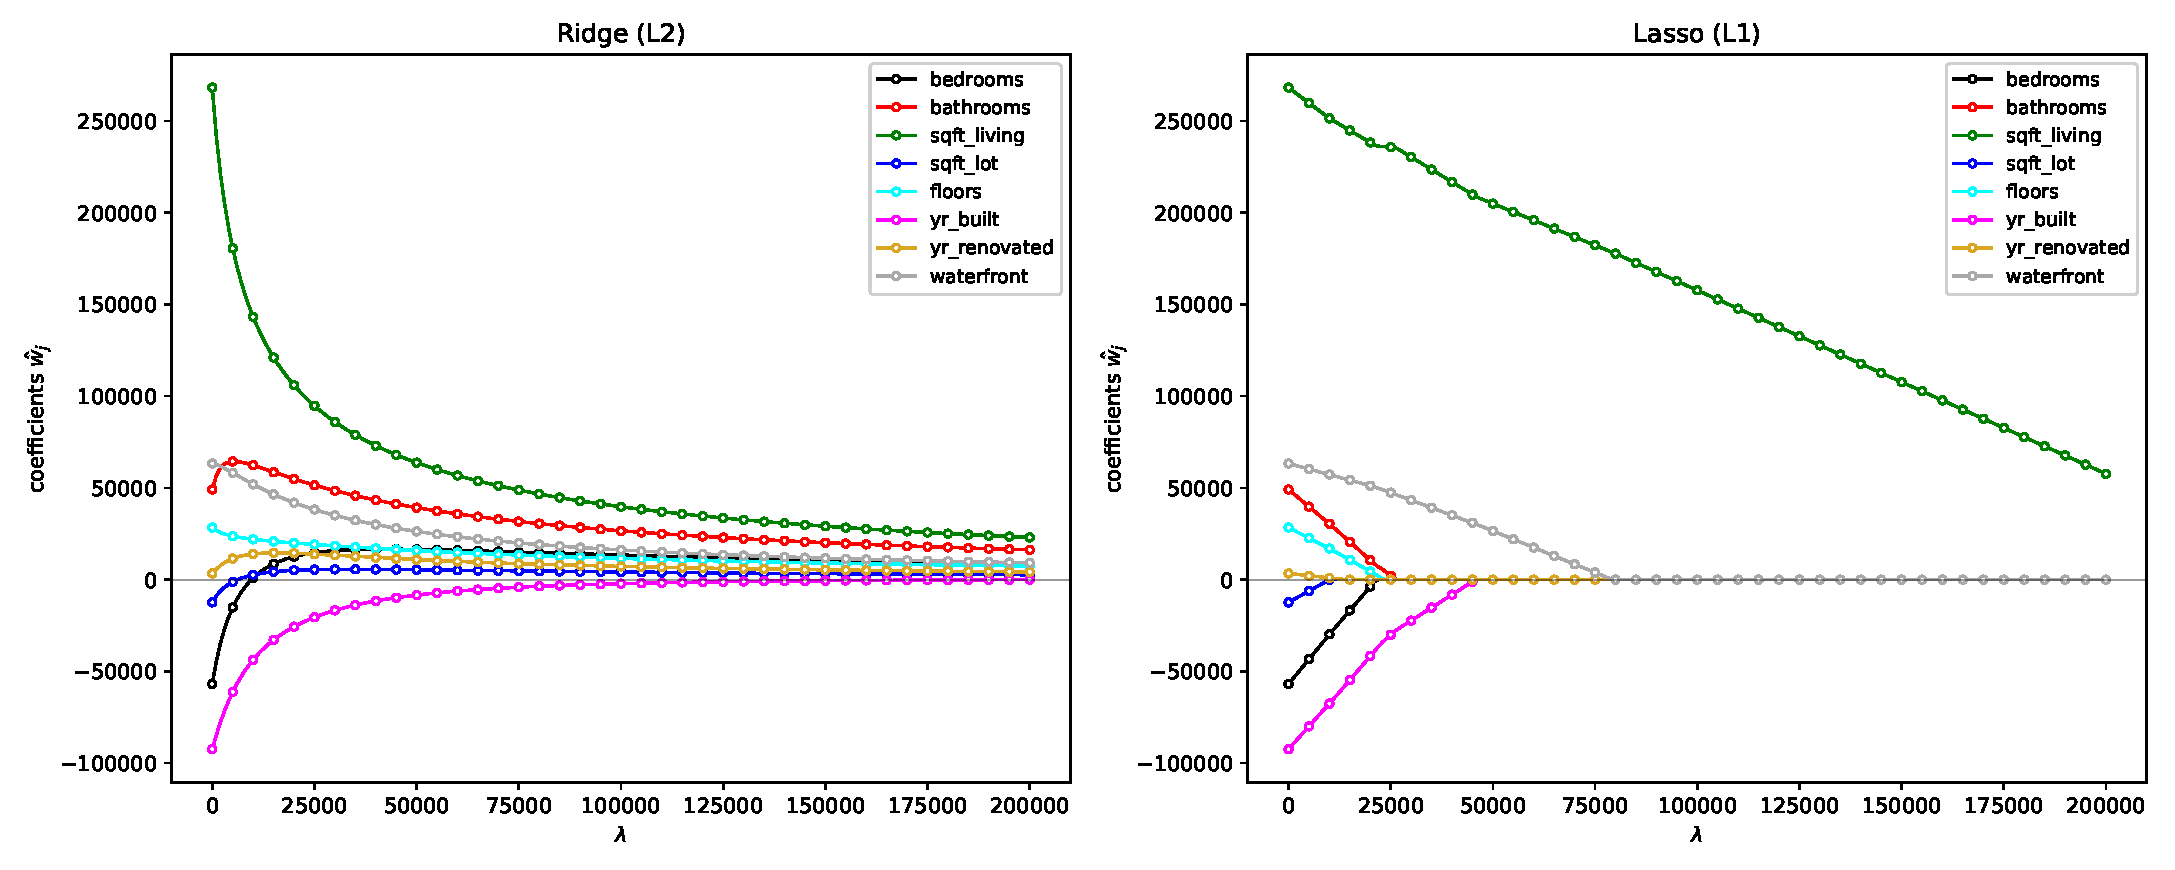
\includegraphics[width=\linewidth]{question/figures/q1_both_paths.pdf}
  \caption{King County 数据（8 特征 z-score、price 中心化）的系数路径。左：Ridge（$\ell_2$）——只缩不归零；右：Lasso（$\ell_1$）——精确归零，sqft\_living 保留到最后。}
\end{figure}


% ======================================================================
\FloatBarrier
\subsection*{2. 用案例说明 $\ell_2$ 阈值化做特征选择为什么不好}

\textbf{题面：}请用案例说明 $\ell_2$ 正则化在回归中将很小的系数设为 0 进行特征选择是不好的（相比 $\ell_1$ 正则化，课件第 44 页）。

\textbf{（1）案例设置。}在 Q1 的 8 列基础上加入 sqft\_above 构成 9 特征（它与 sqft\_living 的相关 $r=0.876$，是最强共线对，两者形成强共线性对），对数据进行标准化后，考察“$|w_j|<\tau$ 视为 0”的阈值化特征选择。

\textbf{（2）阈值化 Ridge 的三个问题。}第一，选择结果高度依赖阈值与路径：同一 Ridge 拟合（$\lambda=2\times10^4$）下，$\tau=10^4\to2\times10^4\to5\times10^4\to10^5$ 对应选中 $7\to5\to2\to0$ 个特征，$\tau=10^5$ 时连 sqft\_living 都被删空；固定 $\tau=10^4$ 沿 $\lambda$ 扫描，保留集跳变 11 次、含 3 次“回升”。相比之下，Lasso 的零模式沿 $\lambda$ 特征数逐渐减少。第二，笔者构造出的共线组被“平摊”后整组删除：预测依赖共线组内两个系数之和，多个系数可能都较小但总体权重较高。例如对于构造的共线组，在 $\tau=10^5$ 下单特征模型保留、9 特征模型两个成员双双被删。为了表现极端情况，笔者用了合成数据（其中两个特征$x_2\equiv x_1$）把机制推到极限：Ridge 精确对半 ，会被删掉整组，而 Lasso 保留一个代表 $(237\,689,\,0)$。

\textbf{（3）原因分析。}阈值化把“收缩量”误当“重要性”：Ridge 的 $\hat w(\lambda)$ 恒非零且连续收缩，大 $\lambda$ 下全体都小，但系数小并不代表不重要；共线时 $|w_j|$ 更不是重要性度量，共线的特征过多就能把每个系数压到阈值之下；$\tau$ 还是人为引入的第二个超参数，没有目标函数可供优化，选择集随 $\tau$、$\lambda$ 与数据扰动跳变。相反，$\ell_1$ 的零来自 KKT 条件与软阈值，特征数沿 $\lambda$ 单调递减、仅由单一超参数控制，对共线组保留一个代表。综上， $\ell_2$ 阈值化做特征选择是不好的，$\ell_1$才是合理的。

\begin{figure}[htbp]
  \centering
  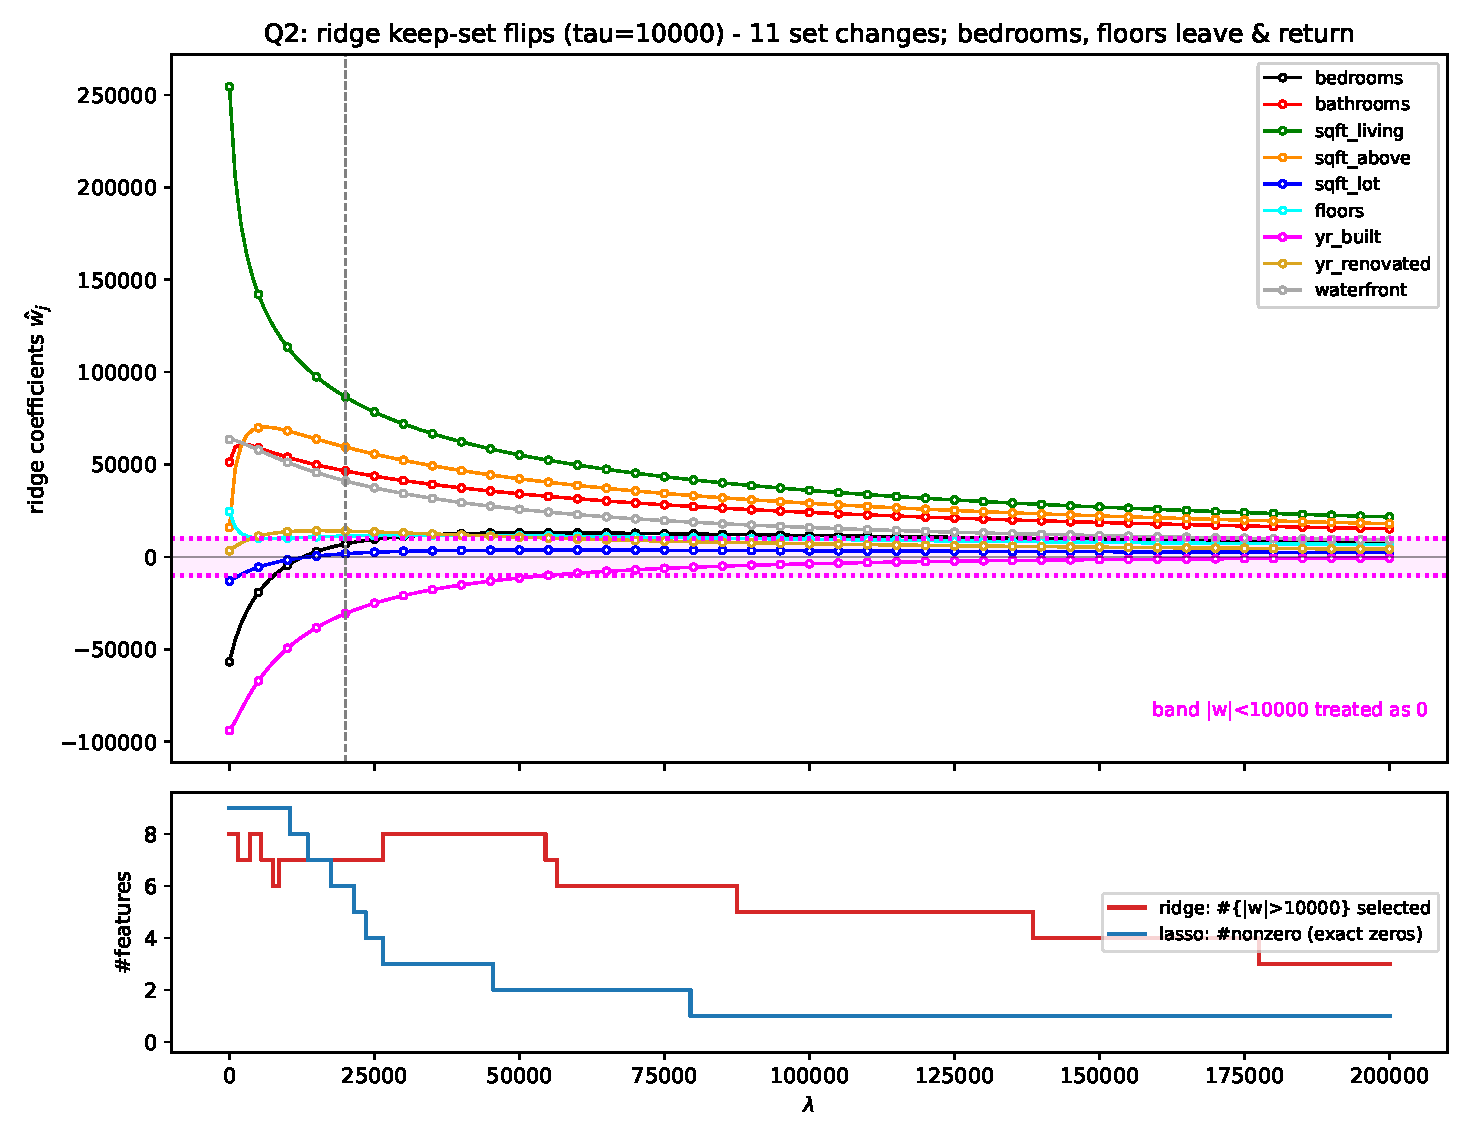
\includegraphics[width=\linewidth]{question/figures/q2_ridge_band_path.pdf}
  \caption{阈值化 ridge 的“选择路径”连单调性都不满足：$\tau=10^4$ 时保留计数沿 $\lambda$ 跳变 11 次（含 3 次回归）；lasso 非零数严格单调。}
\end{figure}

\begin{figure}[htbp]
  \centering
  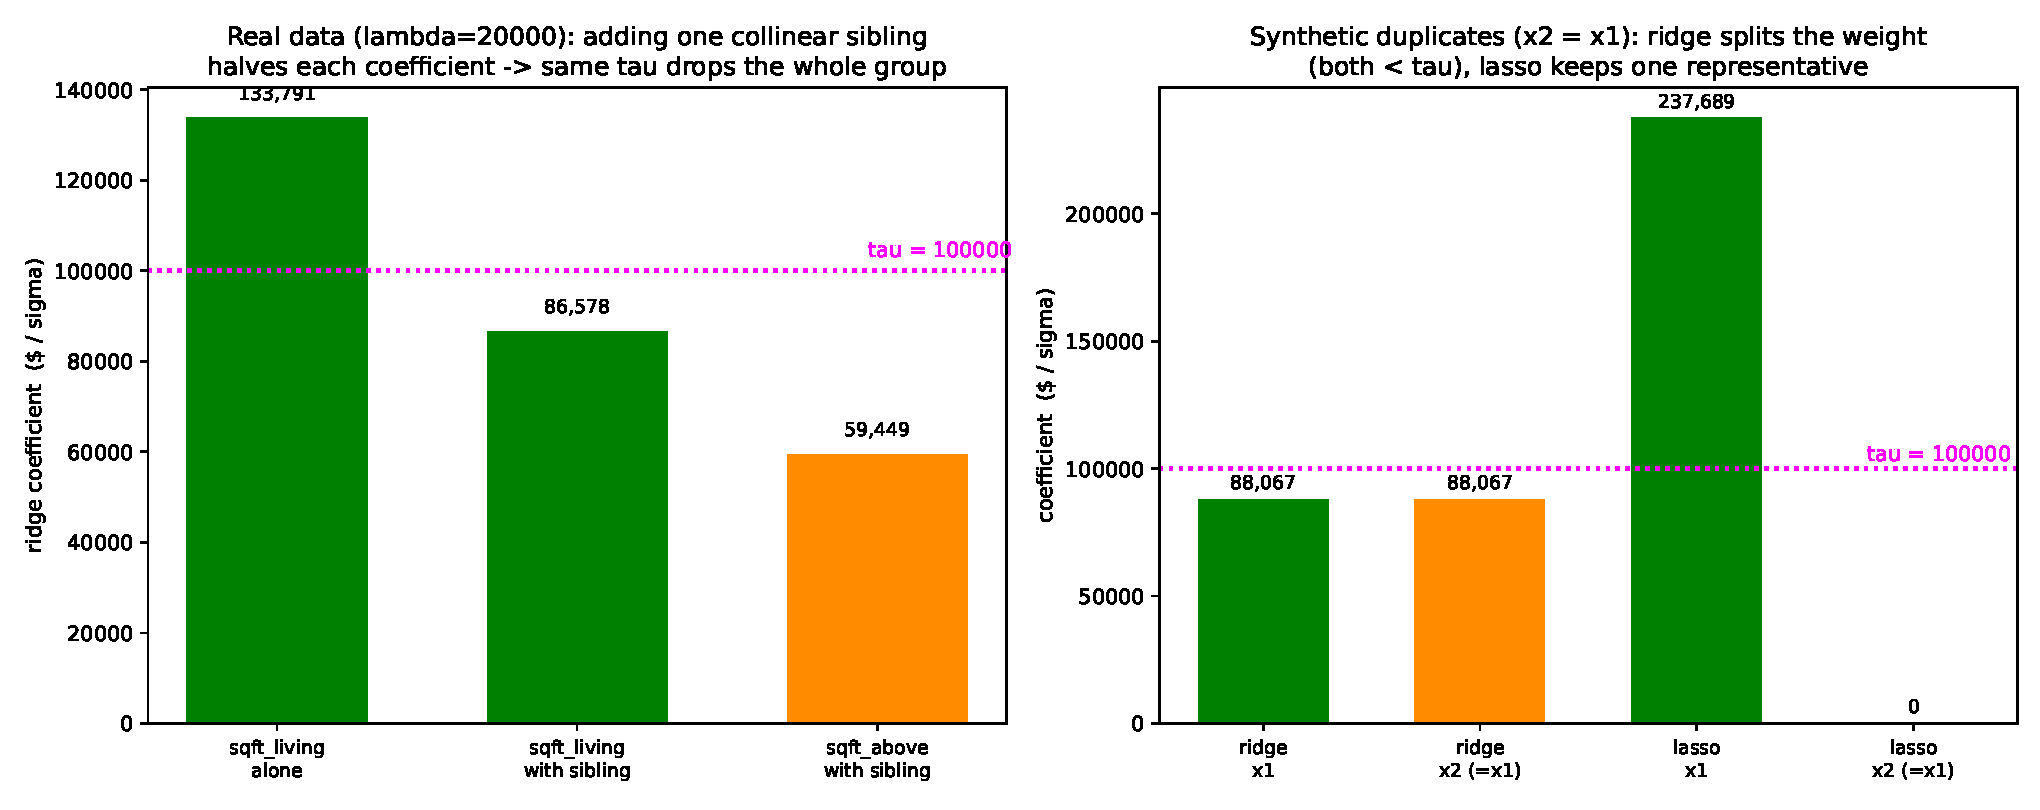
\includegraphics[width=\linewidth]{question/figures/q2_collinear_case.pdf}
  \caption{共线案例：加入一个共线兄弟即可让每个系数减半、$\tau=10^5$ 下整组被删（133\,791 $\to$ 86\,578 + 59\,449）；lasso 组内保留一个代表（237\,689, 0）。}
\end{figure}

\begin{figure}[htbp]
  \centering
  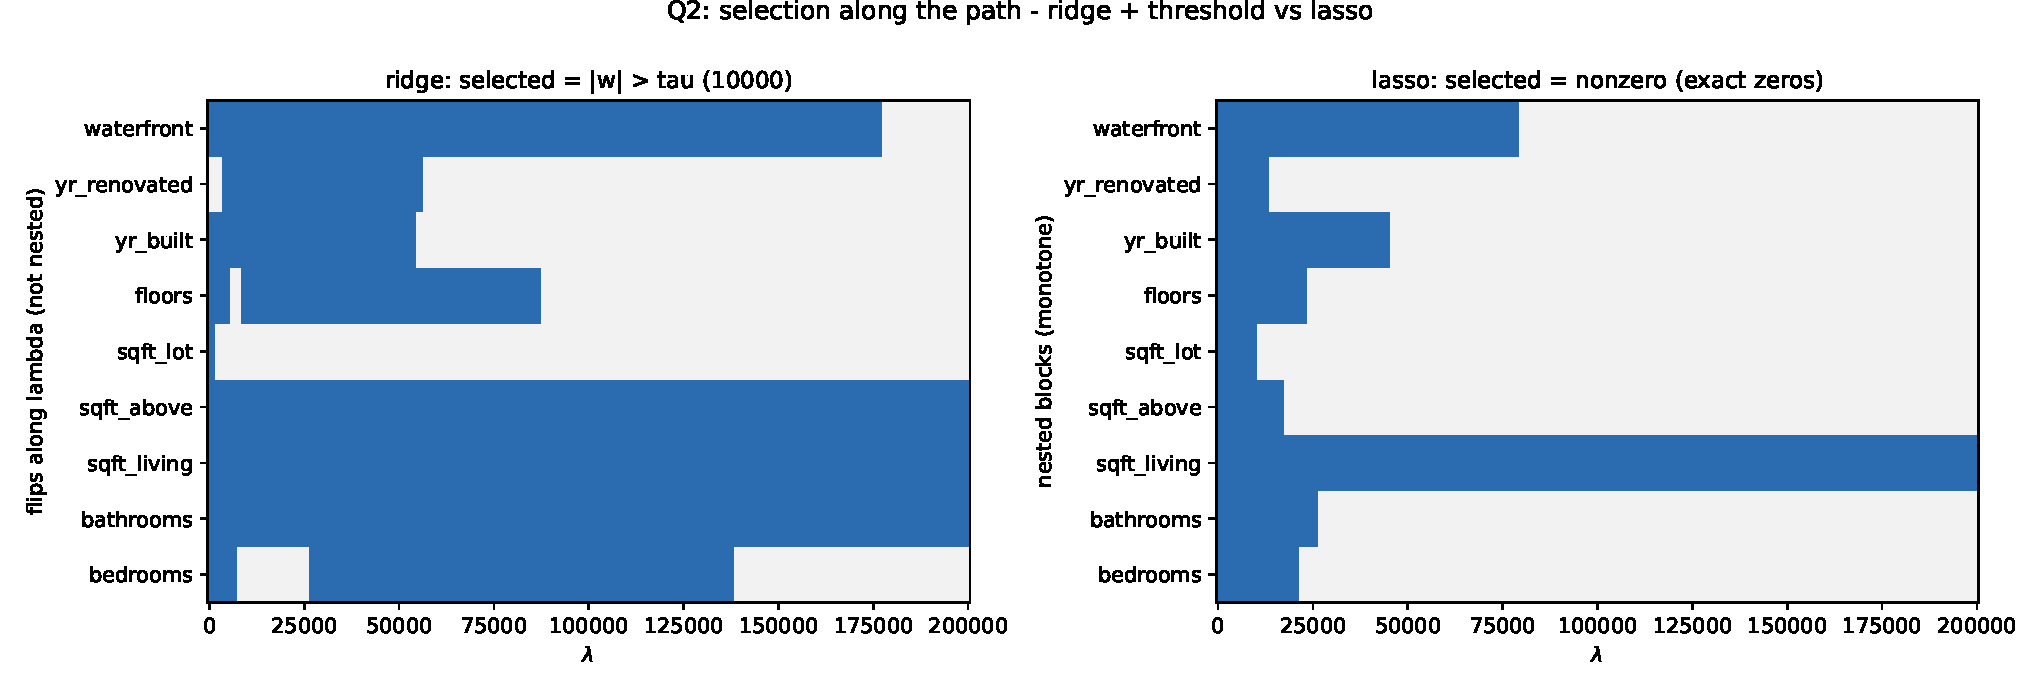
\includegraphics[width=\linewidth]{question/figures/q2_selection_matrix.pdf}
  \caption{结构判据：ridge 阈值化选择集不嵌套（bedrooms、floors 离而复返）；lasso 零模式严格嵌套，每特征仅一个连续非零窗口 $[0,\lambda^*]$。}
\end{figure}

\begin{figure}[htbp]
  \centering
  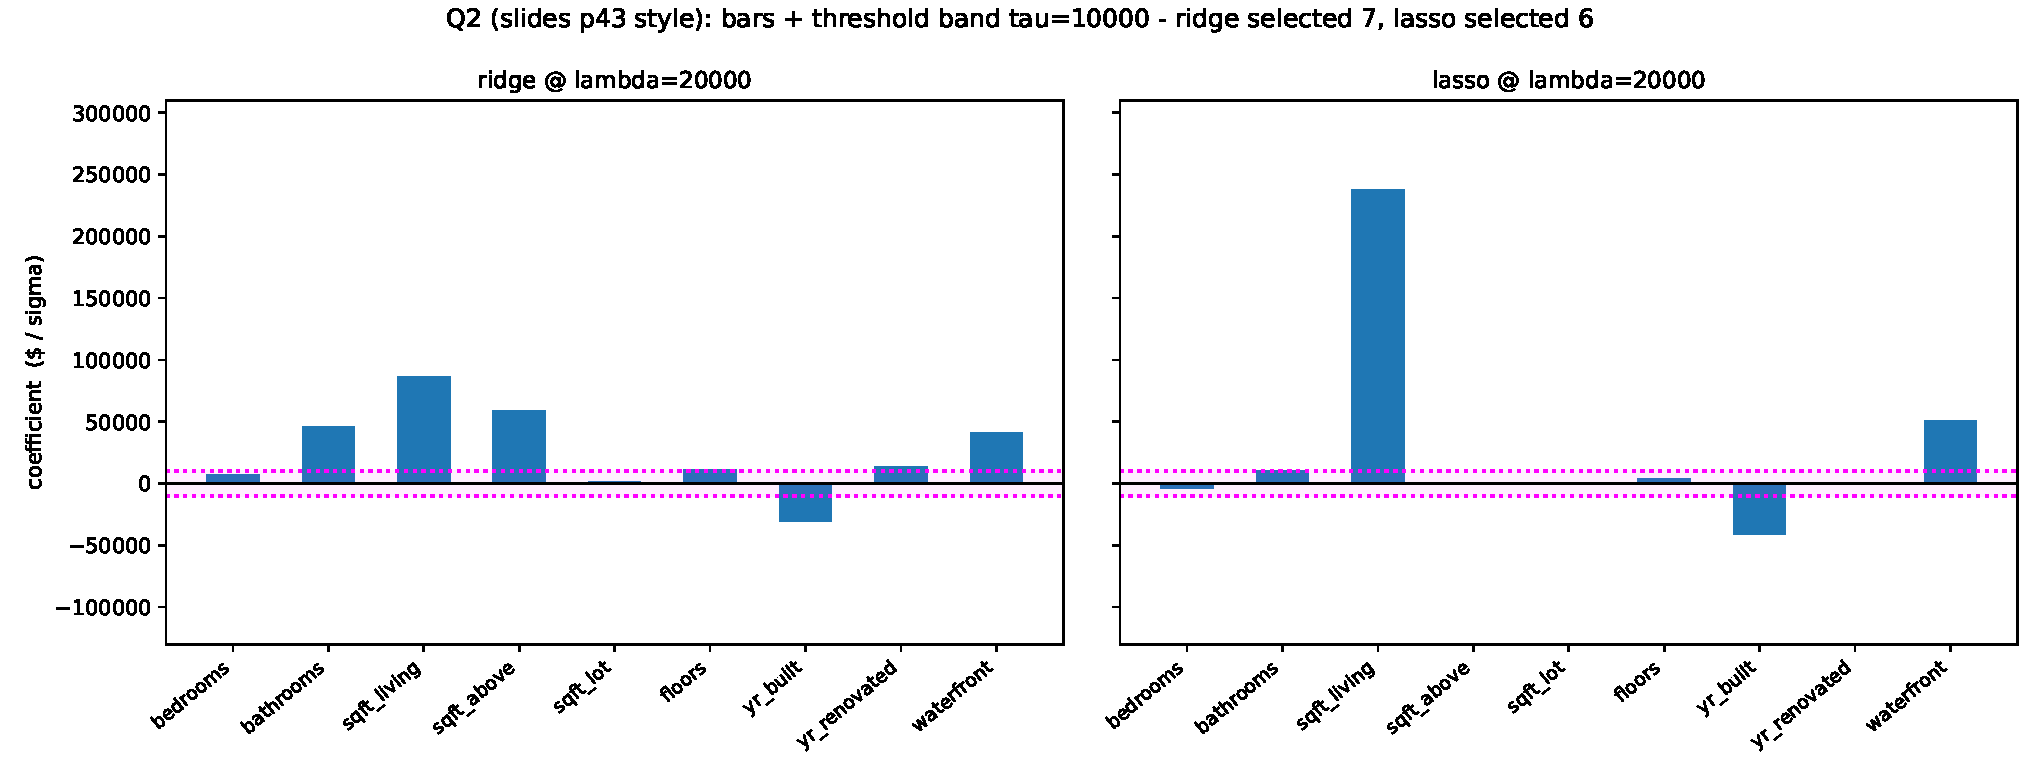
\includegraphics[width=\linewidth]{question/figures/q2_bars_story.pdf}
  \caption{同一 $\lambda=2\times10^4$ 截面（p43 画风）：阈值化 ridge 与 lasso 的保留集在 bedrooms、yr\_renovated、sqft\_above 三个特征上互相矛盾；$\tau$ 从 $10^4$ 扫到 $10^5$，ridge 保留数 $7\to5\to2\to0$。}
\end{figure}


% ======================================================================
\FloatBarrier
\subsection*{3. 与 sklearn 实现有拟合效果差异吗}

\textbf{题面：}你的模型相比于 sklearn 的实现有拟合效果上的差异吗？（简要说明即可）
（提示：可以在做完后两项实验后回答该题。）

\textbf{（1）先把正则对齐。}两边 $\lambda$ 的定义不同，先换算：ours 的目标是 $(1/N)\cdot\mathrm{loss}+\lambda_1\|w\|_1+\lambda_2\|w\|_2^2$；对应 sklearn 的 Ridge $\alpha=N\lambda_2$、Lasso $\alpha=\lambda_1/2$、ElasticNet $\alpha\rho=\lambda_1/2$ 且 $\alpha(1-\rho)=\lambda_2$、逻辑回归 $C=1/(2N\lambda_2)$。不换算就会把“超参不同”当成“实现不同”。

\textbf{（2）结论：没有本质差异，差异在于优化上。}目标函数一样、都收敛后，两边就是同一个解：例如world z-score 的 Ridge 对比 $\cos=1.00000$、relL2 $=0.002$。差别都出在优化上：手写模型的学习率受稳定界限制，需要自行调整；sklearn 用精确求解器；手写的模型轮数有限相当于提前停住，继续训练会向 sklearn 靠拢。

\begin{table}[htbp]
  \centering
  \small
  \begin{tabular}{llrrr}
    \toprule
    行 & 设置（ours 口径） & ours valid & sklearn valid & $\cos$ \\
    \midrule
    \multicolumn{5}{l}{\emph{world（L11，MSE，小者好）}} \\
    A2 & z-score，$\lambda_2=1.0$ & 167.06 & 167.17 & 1.00000 \\
    B1 & raw，无正则，ep20000 & 223.58 & 395.02 & 0.871 \\
    B2 & raw，历史最优，ep2000 & 150.43 & 165.34 & 0.897 \\
    \midrule
    \multicolumn{5}{l}{\emph{truth（L20，准确率，大者好）}} \\
    T1 & 无正则，ep4000 & 0.8867 & 0.8533 & 0.772 \\
    T3 & $\lambda_1=\lambda_2=10^{-3}$，ep5000 & 0.8967 & 0.8600 & 0.712 \\
    \bottomrule
  \end{tabular}
  \caption{ours 与 sklearn 的代表性对比（只列代表性行）。T1 的 sklearn valid 对数损失为 $27.77$（ours $0.255$）；B1 的 sklearn 为精确解，ours 为有限轮早停。}
\end{table}

\begin{figure}[htbp]
  \centering
  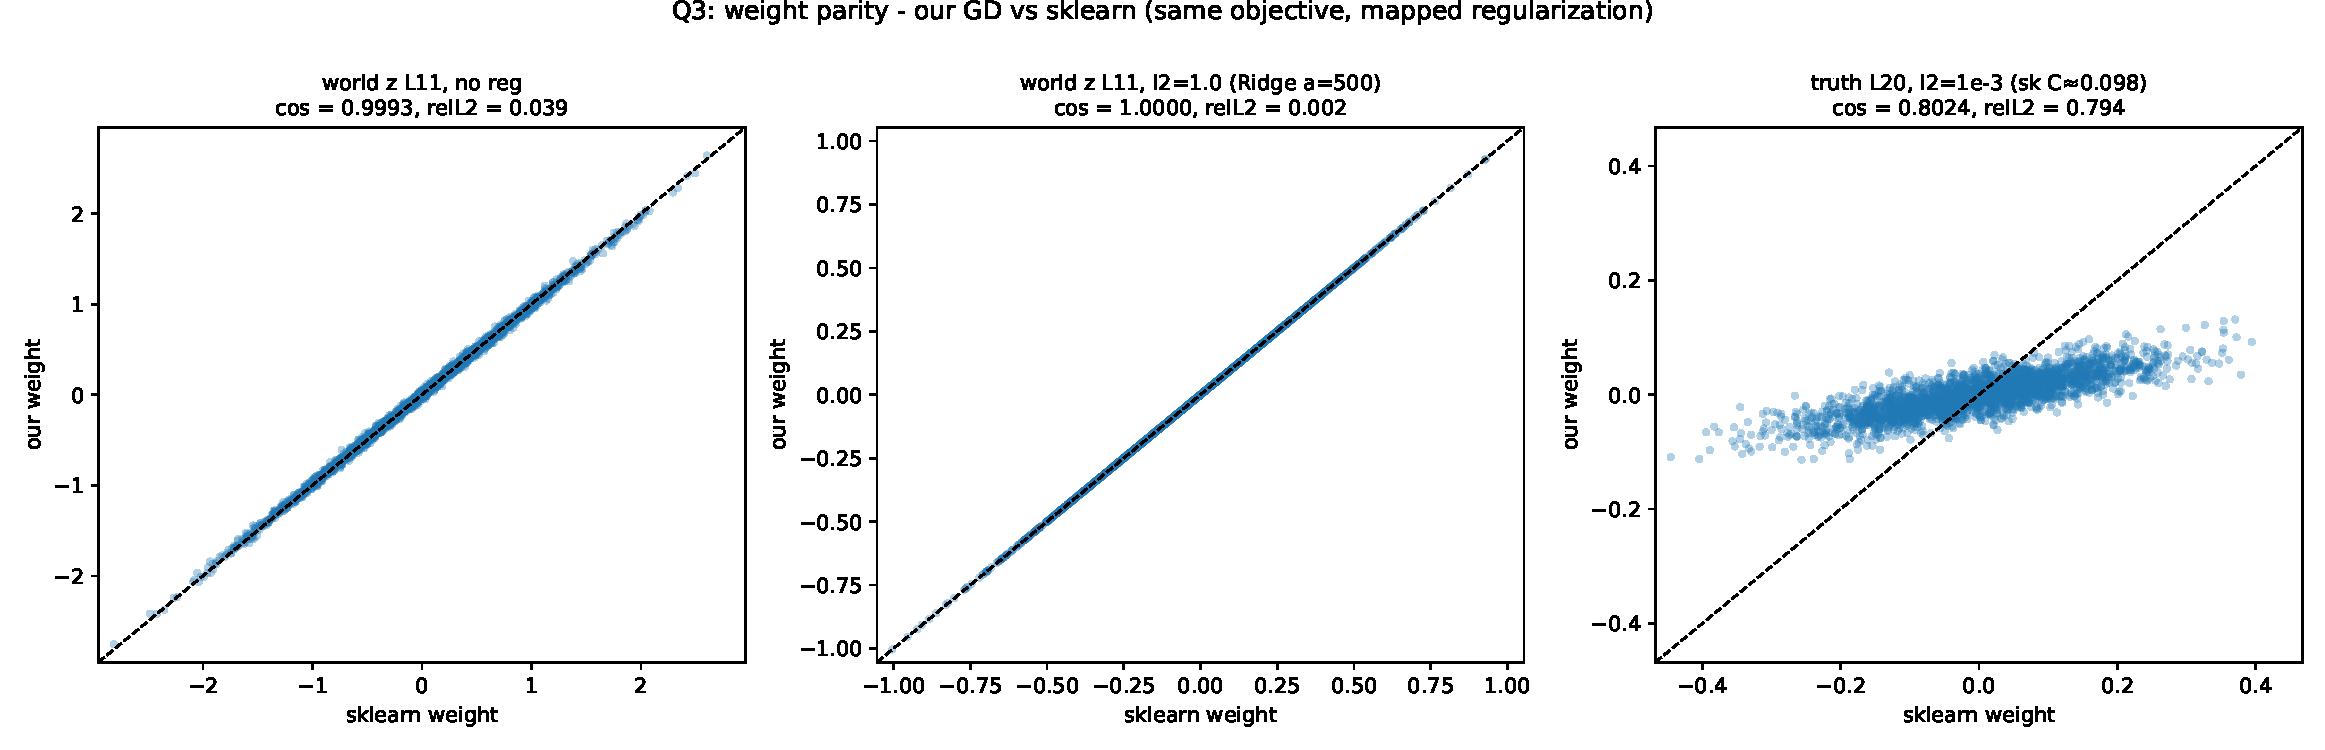
\includegraphics[width=\linewidth]{question/figures/q3_weight_parity.pdf}
  \caption{对齐正则口径后权重逐点比对：world（$\lambda_2=1.0$）落在对角线上（$\cos=1.00000$）——同一目标函数充分收敛 $\Rightarrow$ 同解；truth 未充分收敛时权重整体压向 0（relL2 $=0.794$）。}
\end{figure}


% ======================================================================
\FloatBarrier
\subsection*{4. world：不同层中间表征的预测效果对比与选层}

\textbf{题面：}对比不同层中间表征的预测效果，并分析原因；你在最终模型提交中是如何选择特征选取层次的？

\textbf{（1）实验设置。}实验提供了11，23，35共3层，笔者以3为间隔提取了另外十层，共计13 层（$2,5,\dots,35$）。由于实测时发现不同层按照统一的超参数会出现loss inf现象，所以对数据做了标准化，最后再把权重折算回去。采用了同一套配置做对照：lr$=0.002$、2000 轮、$\lambda_2=1.0$、$\lambda_1=10^{-3}$。

\textbf{（2）结果分析。}曲线呈 \textbf{倒 U 形}：浅层 L2–L11 差异不显著，中层 L14–L29 明显更差（L17/L20/L23 显著），深层 MSE 先降后升。std 中最低为 L2（157.57），但与 L5/L8/L11 差异不显著；全场最低为 raw L11（150.43）——world 水平锁定在 $150$–$167$（$R^2\approx0.955$），继续调参并未发现显著收益。

\textbf{（3）原因分析。}world 的目标是位置坐标，这类信息在浅层表征中最接近线性可分；随层深增加，表征经过更多非线性变换、语义抽象增强，坐标的线性可读性下降，中层出现低谷。深层在 L29–L32 段 MSE 下降（L32 为局部最低 180.31），随后 L34/L35 又回升；下降的可能原因是深层把位置重新编码为更全局的线性方向。

\textbf{（4）最终选层。}提交选中 \textbf{L11}，有三个原因：一是 L11 与 L2/L5/L8 差异并不显著（可以参见表2），L2虽然略微好一点但是与L11差异不大；二是 L11 是实验本身提供的，与实验本身关联性更好；三是标准化一定程度上影响了2，5，8，11四层之间细微的差距，例如笔者对 L2 和 L11 在不进行标准化、统一超参数做了训练，发现 L11 略微优于 L2。综上所述，笔者选择11层作为最终选层。

\begin{figure}[htbp]
  \centering
  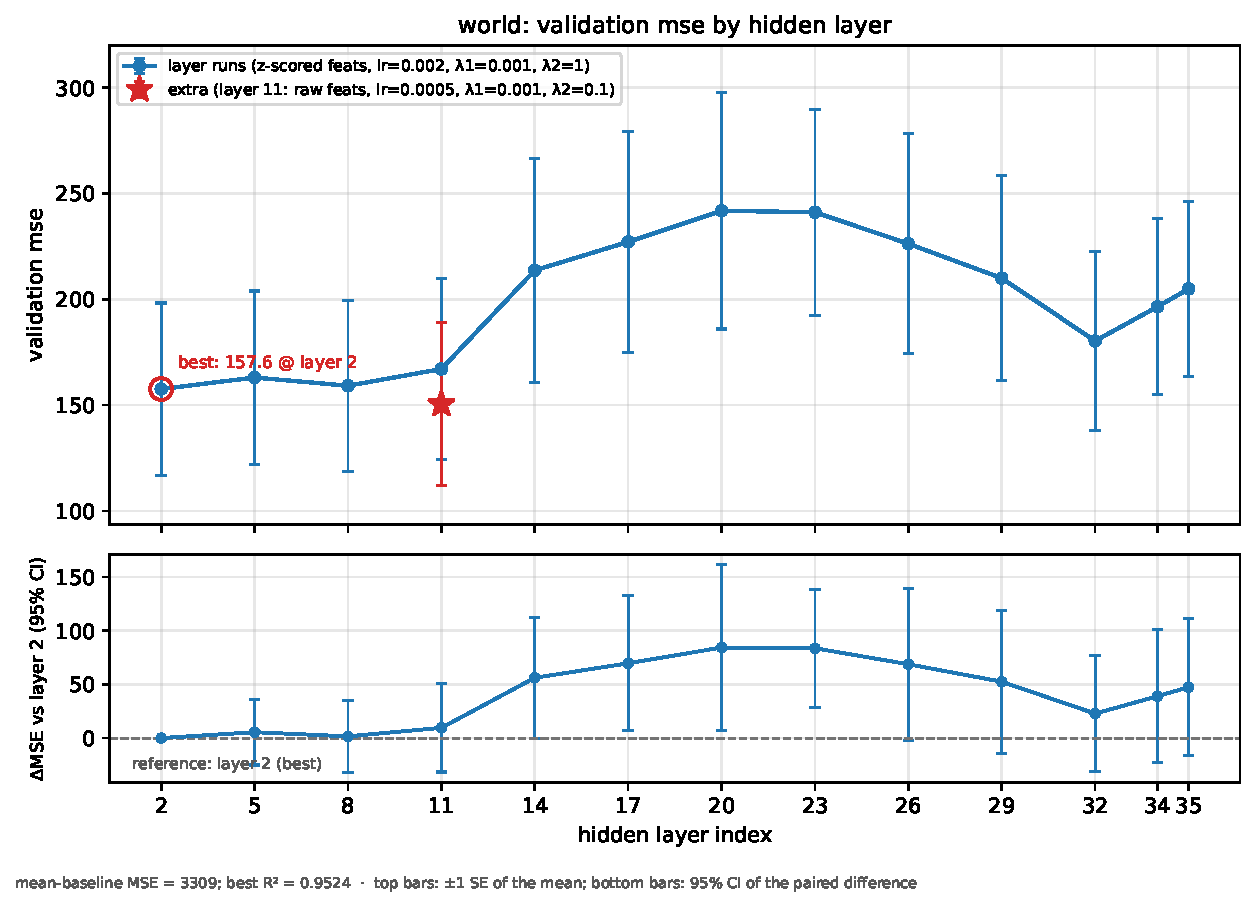
\includegraphics[width=\linewidth]{results/slurm_layers/world/plots/world_layers.pdf}
  \caption{world 各层验证 MSE（上：$\pm1$ SE，红圈 = 最优 std 层，红星 = raw L11 extra；下：与 L2 的配对差 95\% CI）。浅层平台—中层低谷—深层回升的倒 U 形。}
\end{figure}

\begin{table}[htbp]
  \centering
  \small
  \begin{tabular}{rrrrrl}
    \toprule
    层 & 配置 & MSE & $\pm$SE & $\Delta$ vs L2（95\% CI） & 判定 \\
    \midrule
    2 & std & \textbf{157.57} & 40.7 & 参考 & 最优 \\
    5 & std & 163.02 & 40.9 & $+5.4\pm30.5$ & 不显著 \\
    8 & std & 159.14 & 40.5 & $+1.6\pm33.5$ & 不显著 \\
    11 & std & 167.04 & 42.9 & $+9.5\pm41.1$ & 不显著 \\
    14 & std & 213.67 & 53.1 & $+56.1\pm56.2$ & 边缘 \\
    17 & std & 227.13 & 52.4 & $+69.6\pm62.7$ & 显著 \\
    20 & std & 241.83 & 55.9 & $+84.3\pm76.9$ & 显著 \\
    23 & std & 241.14 & 48.6 & $+83.6\pm54.8$ & 显著 \\
    26 & std & 226.25 & 52.0 & $+68.7\pm70.8$ & 边缘 \\
    29 & std & 209.99 & 48.3 & $+52.4\pm66.5$ & 不显著 \\
    32 & std & 180.31 & 42.1 & $+22.7\pm54.1$ & 不显著 \\
    34 & std & 196.46 & 41.6 & $+38.9\pm61.9$ & 不显著 \\
    35 & std & 204.91 & 41.5 & $+47.3\pm63.9$ & 不显著 \\
    11 & raw（extra） & \textbf{150.43} & 38.4 & — & 全场最低 \\
    \bottomrule
  \end{tabular}
  \caption{world 13 层验证 MSE 全表（含 raw extra）。}
\end{table}


% ======================================================================
\FloatBarrier
\subsection*{5. world：正则化与学习率的选择}

\textbf{题面：}你在最终模型提交中是怎么选择正则化的？请说明理由；

\textbf{（1）为什么正则化？}world 是 $N=500$、$D=2560$，样本远少于维度，本身是一个欠定问题，必须正则化。默认的对照设置为 lr=0.003, epochs=2000, λ1=0.001，λ2=1, layer=11。

\textbf{（2）正则扫描。}固定其他，扫 $\lambda_2$：$0.1$ 时训练残差已经很小（$\approx3$），但 valid MSE 209，明显过拟合；$1.0$ 最好（$167.06$）；$3.0$ 正则强度过高，MSE回升到 $184.57$。把 $\lambda_1$ 从 $0$ 扫到 $0.1$，valid MSE 只从 $167.07$ 降到 $165.82$，差异不显著，所以后续沿用 $10^{-3}$。

\textbf{（3）学习率扫描。}学习率在稳定界内选（见后面对稳定界探索的说明），再用训练表现验证：原始的 L11 的稳定界是 $3.6\times10^{-3}$，取 lr$=5\times10^{-4}$，$1\times10^{-3}$，$2\times10^{-3}$，$5\times10^{-3}$。结果来看lr$=5\times10^{-3}$结果最好，故选择 lr$=5\times10^{-3}$。

\textbf{（4）最终提交。}最终模型的提交是\textbf{raw L11}，超参数为lr$=5\times10^{-4}$、2000 轮、$\lambda_2=0.1$，valid MSE \textbf{150.43}。选择理由见上面的分析，以及后面的图。

\begin{figure}[htbp]
  \centering
  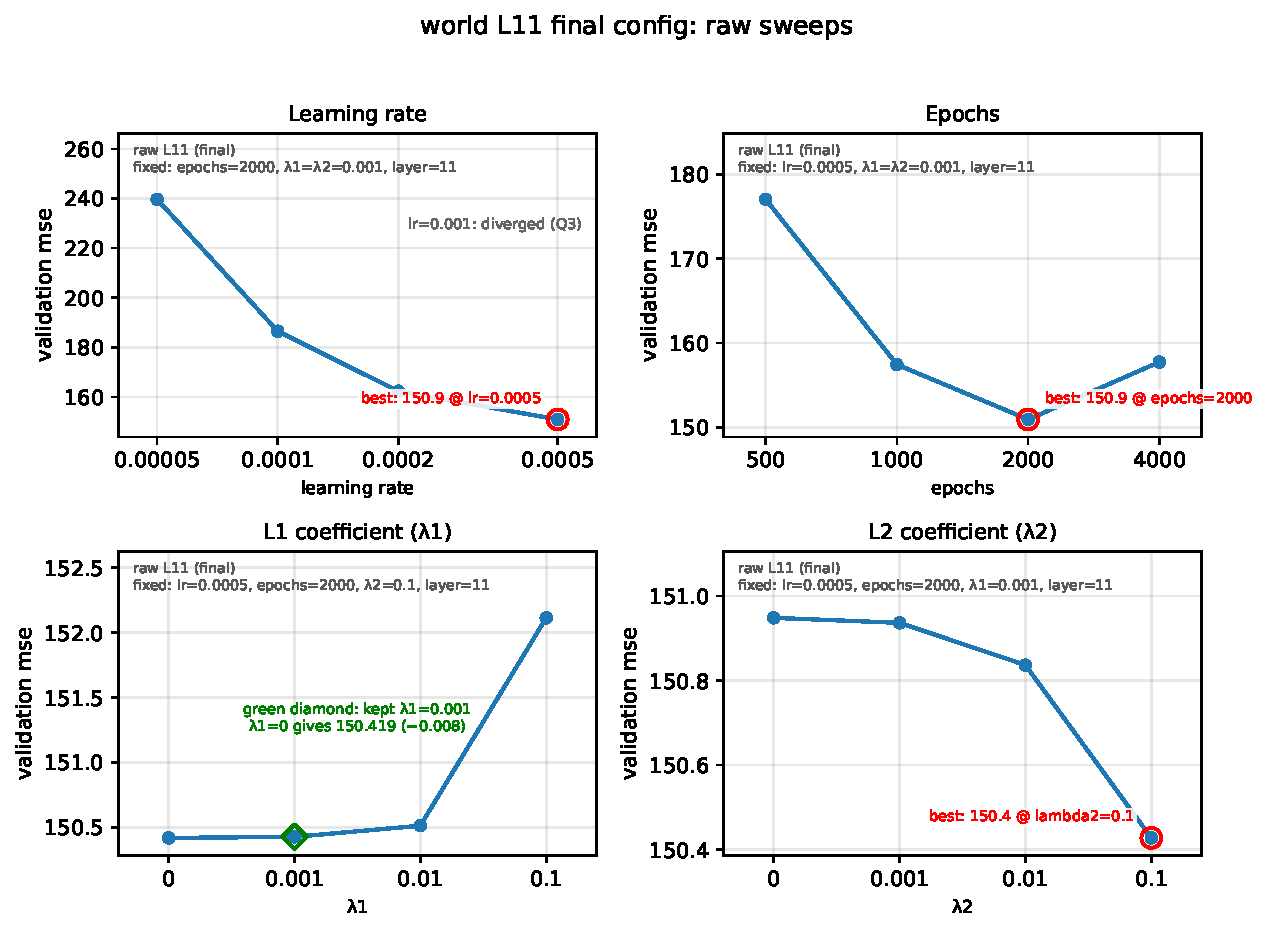
\includegraphics[width=\linewidth]{results/q5_grid/plots/world_grid.pdf}
  \caption{world L11 的 raw 单变量扫描（各格只变一个超参，基线见图内 fixed 小字；最终提交为 lr$=5\times10^{-4}$、2000 轮、$\lambda_1=10^{-3}$、$\lambda_2=0.1$）：lr 在 $5\times10^{-4}$ 最低（150.9），$10^{-3}$ 已发散（第 3 题）；epochs 在 2000 轮最低（150.9）；$\lambda_1$ 四点为 150.42/150.43/150.51/152.11，$0$ 仅低 0.008，取 $10^{-3}$ 保留弱正则；$\lambda_2$ 在 $0.1$ 最低，对应提交权重 150.4277。}
\end{figure}


% ======================================================================
\FloatBarrier
\subsection*{6. 验证集预测的地图可视化}

\textbf{题面：}给出你的模型在验证集上的预测结果，并可视化在地图上（推荐不含国界线）。
（提示：此题推荐使用 AI 工具辅助可视化程序的编写。）

\textbf{（1）绘图数据来源。}图和读数都基于最终提交的 world raw L11 权重。

\textbf{（2）地图读数。}130 个验证样本（78 国）画在世界地图上：灰空心圆是真值，彩点是预测，颜色表示单点误差 $\sqrt{\Delta lat^2+\Delta lon^2}$。

\textbf{（3）数据分析。}模型大致学到的是“大洲级”定位：平均误差 $12.44^\circ$、中位 $9.52^\circ$（大圆距离约 $953.8$ km），四分位 $4.96/9.52/15.34^\circ$，误差超过 $30^\circ$ 的只有 $7/130$。

\textbf{（4）误差分析。}误差呈现出两个特点。第一，方向不对称：纬度平均只差 $4.25^\circ$，经度差 $10.85^\circ$，约 2.5 倍。第二，见过的地方准、偏僻的地方差：欧洲、东非、中美等训练密集区误差普遍小于 $5^\circ$（最准 Denmark $0.79^\circ$）；失败集中高纬和孤立岛屿——两条南极样本排在最差前二（$89.6^\circ$、$73.8^\circ$，预测落到约 $28$–$34^\circ$E 的南大洋），纽芬兰样本纬度几乎全对（差 $0.23^\circ$），经度却差了 $40.7^\circ$。图上只画 110m 海岸线，\textbf{不含任何国界线}。

\begin{figure}[htbp]
  \centering
  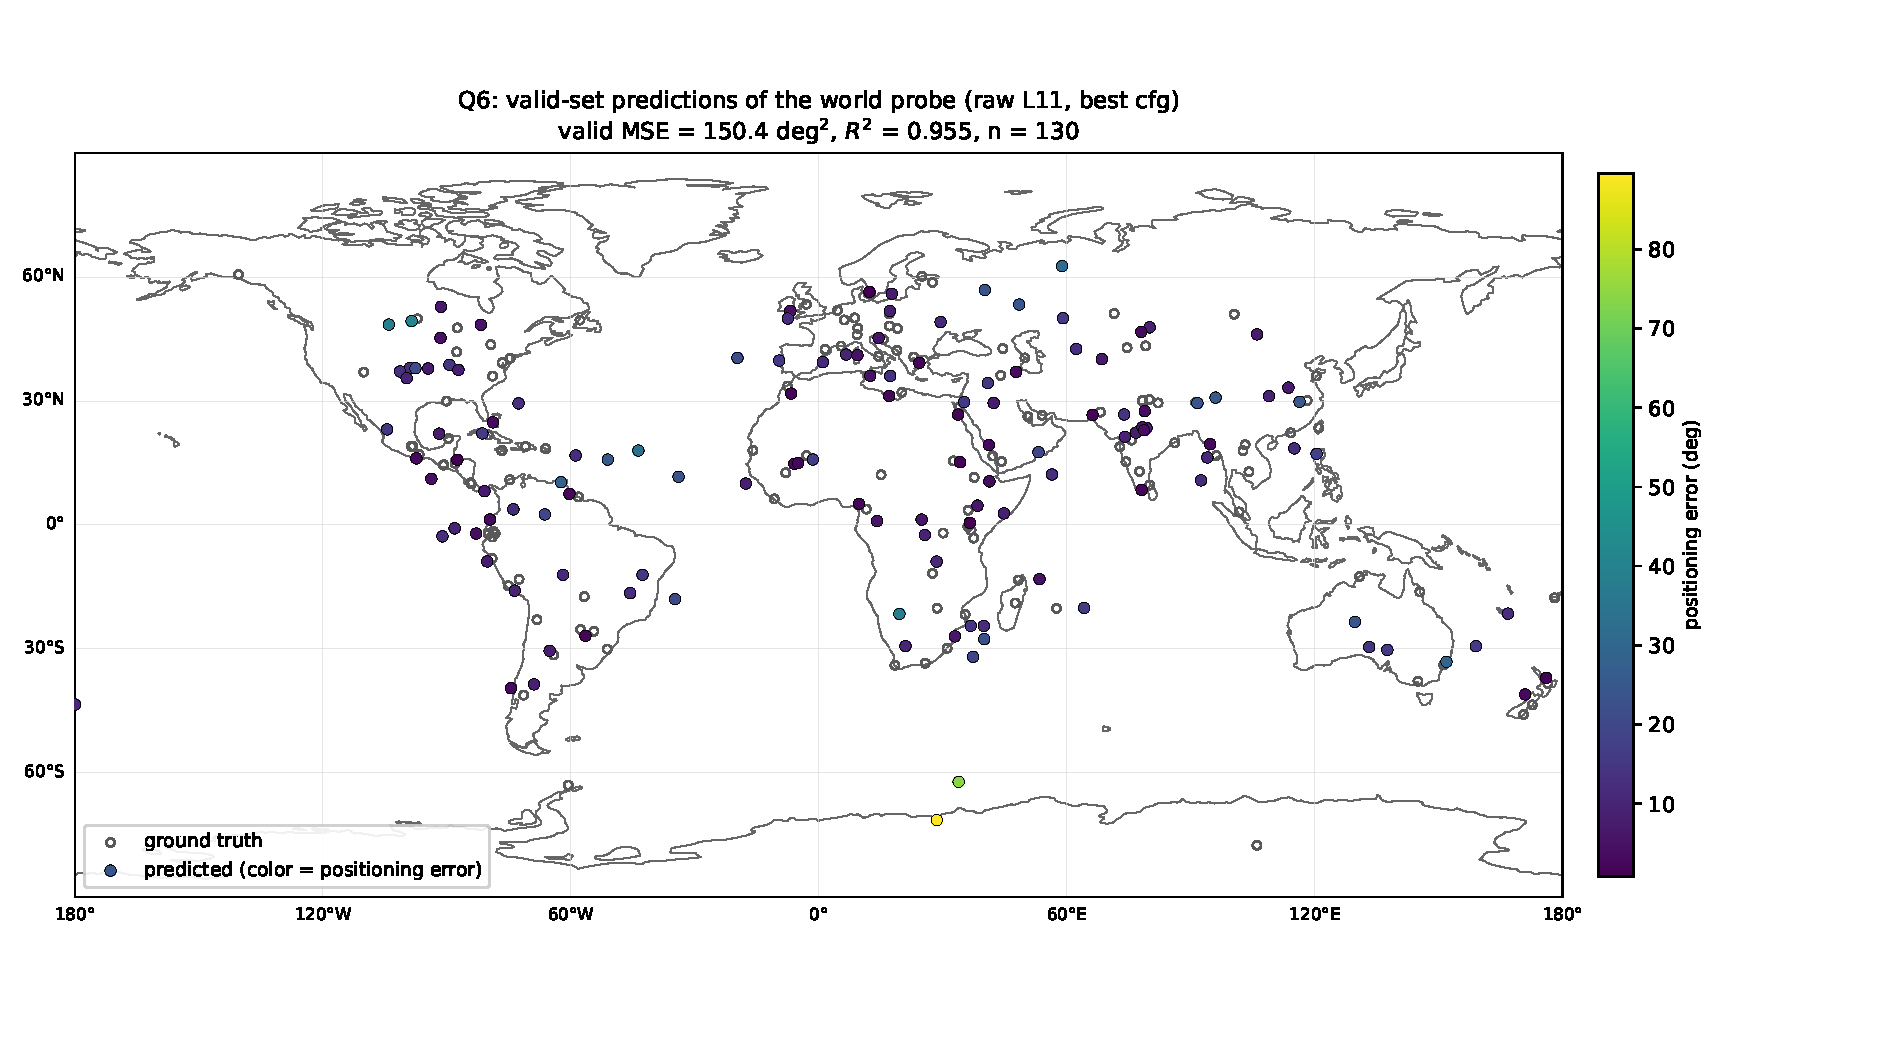
\includegraphics[width=0.85\linewidth]{question/figures/q6_valid_map.pdf}
  \caption{130 个验证样本的定位：灰空心圆 = 真值，彩点 = 预测（颜色 = 单点定位误差）。valid MSE $=150.4$（$R^2=0.955$）；中位误差 9.5$^\circ$，纬度误差显著小于经度；高纬与孤立岛屿样本误差最大。仅海岸线，无国界线。}
\end{figure}


% ======================================================================
\FloatBarrier
\subsection*{7. 是地理坐标表征，还是仅仅识别了国家？}

\textbf{题面：}从训练集和验证集的表现，是否能够强烈说明模型内部存在地理坐标的表征，而不是仅仅识别了输入中的国家？对于该题可以参考原始论文 [3] 的部分结论和上一题的可视化结果；也可与按训练集国家分组的平均坐标基线比较，考察同一国家内不同地点的预测。

\textbf{（1）判据与基线。}如果模型只是认出了国家，那么把“该国平均坐标”直接告诉它，效果应不差于模型。所以主基线用 \textbf{oracle 国家均值}：按真实国家标签查训练集里该国坐标的均值（等于给真标签 $+$ 训练记忆），未见国家退回全局均值；分层 all 130 / seen 110 / multi 73 / single 37 / unseen 20，improvement $=$ 基线 $-$ 模型，置信区间用 paired bootstrap。

\textbf{（2）证据：有位置信息，但很弱。}unseen 的 20 条在训练中完全没出现，按国家查表原理上不可能：模型 MSE $158.90$，全局均值基线 $1182.83$，improvement $\mathbf{+1023.93\ [513.94,\ 1654.14]}$——模型仍把样本放到正确的大洲/区域。但全局均值基线本身很弱，这只说明“模型远不止一个全局平均”，不说明“模型精确”。限定到见过的国家，oracle 反而反超：seen 110 条上模型 $148.89$ vs 基线 $\mathbf{113.77}$（imp $-35.12\ [-60.90,\ -7.08]$），multi 同向（$205.0$ vs $159.6$），single 不显著；同国 73 条多样本样本相对本国训练均值的纬度相关 $r=0.201\ [0.021,\ 0.389]$（弱显著），经度 $r=0.046$（不显著）。可见模型确实带了超出国家身份的位置信息，但精细定位能力有限。

\textbf{（3）结论：中等强度。}unseen 的预测整体落对区域（欧洲$\to$欧洲、中美$\to$中美），最差 Mauritius $38.03^\circ$、最好 Denmark $0.79^\circ$，失败模式与 Q6 一致（经度、岛屿）。综合看，证据强于“纯国家分类器”，弱于论文 [3] §5 的神经元 $+$ 干预级别，与论文 §4.1 的 “weak evidence” 自评、课程 README “可解码 $\neq$ 生成时一定使用” 的提醒一致；Q6 地图上经度和岛屿的大误差正是 “relative position correct, absolute position often wrong” 的具体表现。

\begin{figure}[htbp]
  \centering
  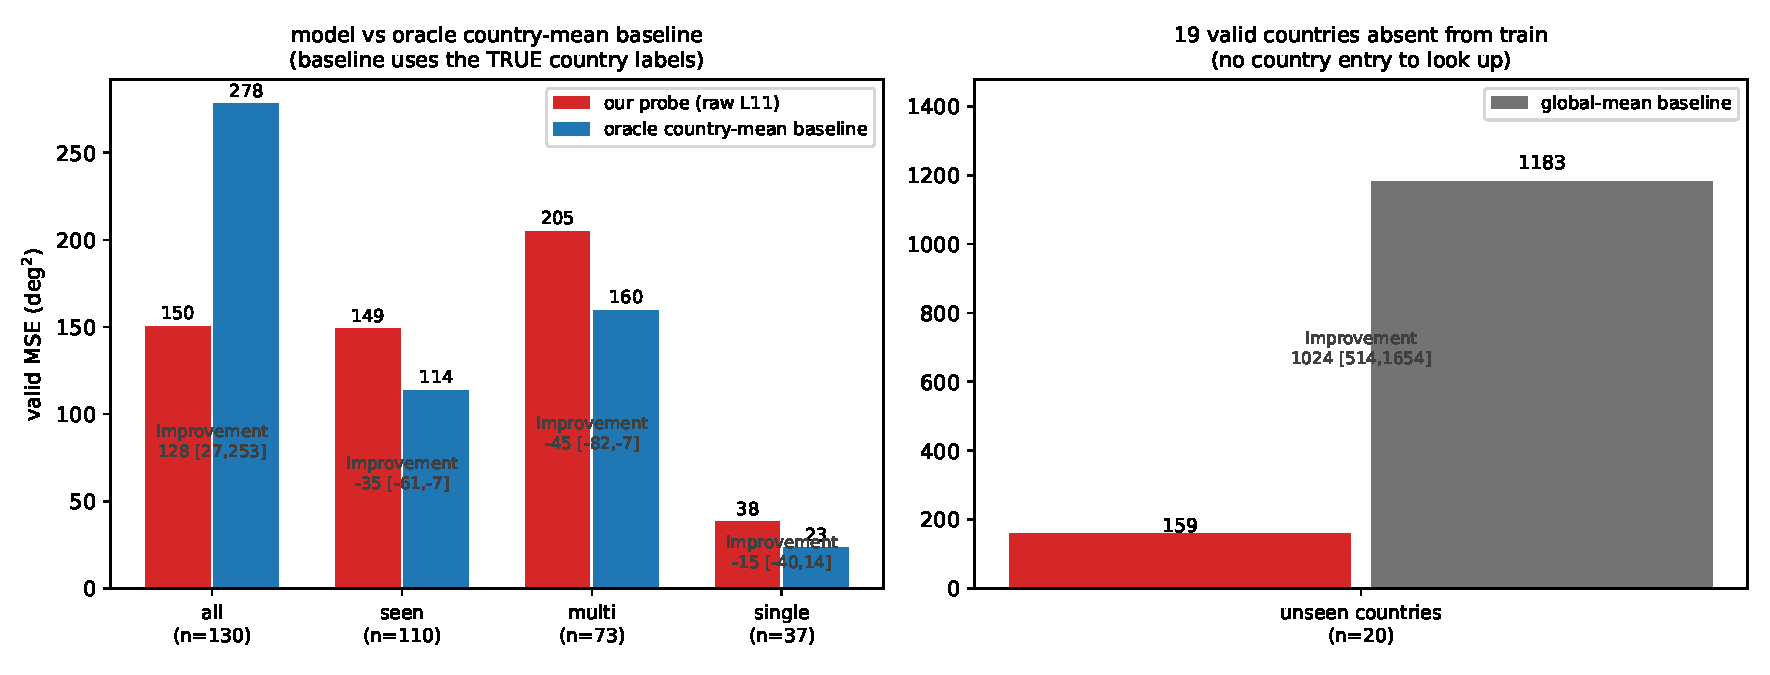
\includegraphics[width=\linewidth]{question/figures/q7_baseline_bars.pdf}
  \caption{模型 vs oracle 国家均值基线的分层 valid MSE。左：seen 国家按样本数分层；右：19 个训练未见国家。improvement $=$ 基线 $-$ 模型；误差棒为 paired bootstrap 95\% CI。}
\end{figure}

\begin{figure}[htbp]
  \centering
  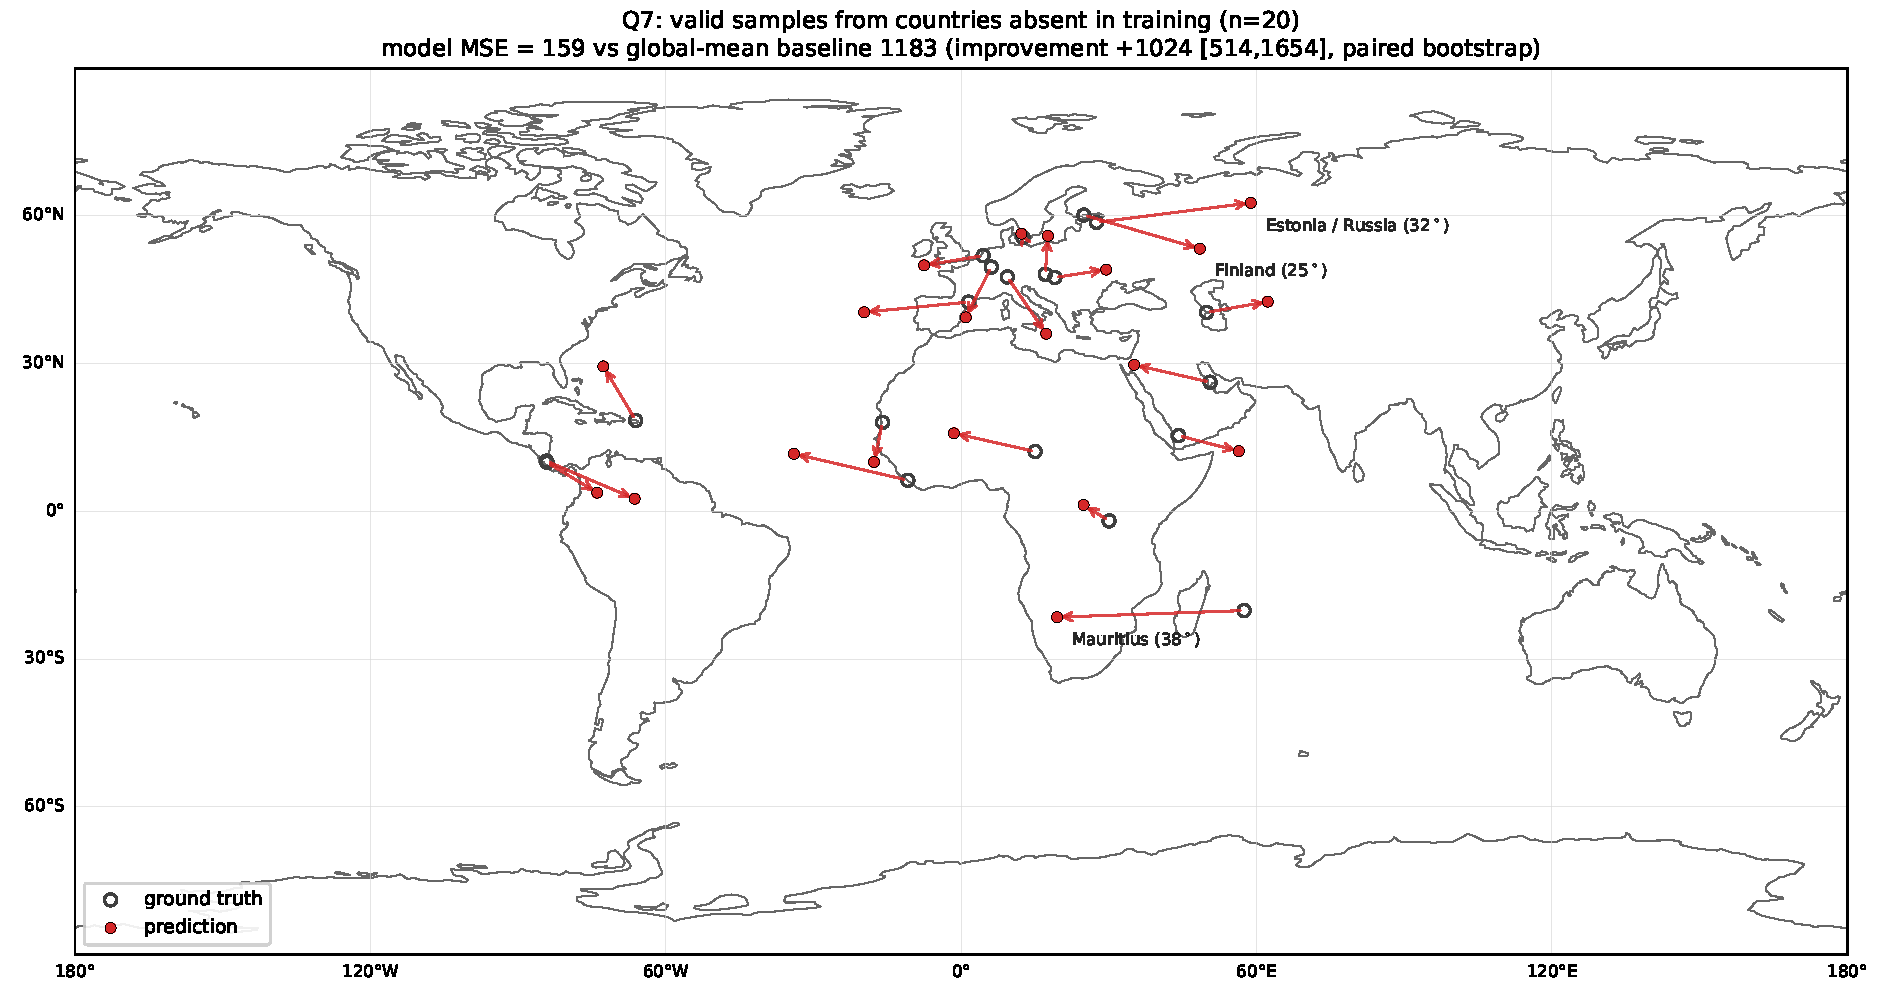
\includegraphics[width=\linewidth]{question/figures/q7_unseen_map.pdf}
  \caption{19 个未见国家 20 条样本：模型 MSE 159 vs 全局均值基线 1183（imp $+1024$）。预测整体落对区域（欧洲$\to$欧洲、中美$\to$中美），最差 Mauritius 38.0$^\circ$。仅海岸线，无国界线。}
\end{figure}


% ======================================================================
\FloatBarrier
\subsection*{8. truth：训练集/验证集的分布差异与应对}

\textbf{题面：}仔细阅读训练集和验证集，模型的训练集和验证集存在哪些分布上的差异？你是如何应对的？

\textbf{（1）分布差异。}主要有三点。① \textbf{拼写噪声}：train 有 $7.0\%$（$354/5088$）的句子带相邻字母交换型错拼（mkaes$\to$makes 这种），valid 有 $24.7\%$（$74/300$），约为 train 的 $3.5$ 倍，但在两类标签内都均衡。② \textbf{主体新颖度}：valid 的 212 条可识别首实体中，164 条（\textbf{77.4\%}）在 train 里没出现过；从 train 随机抽 300 条做同样统计，零假设只有 $20.8\%\ [15.6,\ 25.6]$，valid 远在分布之外。③ \textbf{模板/长度}：train 特有的 “One can”/“If one” 句式约 $3.0\%$，valid 只剩 $0.7\%$；valid 的长句被截断（最长 $162$ vs $487$ 字符）。核心差异是“噪声 $+$ 新主体”。

\textbf{（2）对模型的影响。}L20 总体 $0.8967$。带错拼的子集 $0.932\ [0.865,0.986]$，不比干净子集 $0.885\ [0.841,0.925]$ 差，差 $-0.047\ [-0.115,+0.024]$（CI 含 0）；主体 seen $0.917$ 对 unseen $0.884$，差 $+0.033\ [-0.063,+0.119]$，同样不显著——两类“难样本”都没有明显掉分。逐层看，错拼只在浅层造成伤害：L5–L11 的干净$-$错拼差为 $+5\sim7$pp，L17 起转负（L20 为 $-4.7$pp），说明文本噪声在中深层被平滑吸收了。

\textbf{（3）应对。}第一，读数方式：子集比较都配 bootstrap 95\% CI（$n=300$ 的单点差异约 $\pm3.5$pp），CI 跨 0 就不用它们来选层/选参，并分层报告而不是只看总 acc。第二，不向 valid 泄漏：层和超参来自扫描、配对检验，训练预算固定，不按 valid 早停。第三，文本不清洗：特征直接从原始文本（含错拼）前向——如果清洗 train 侧的错拼，train（$7.0\%$）和 valid（$24.7\%$）的口径反而更不一致，而且部署时同样要面对噪声；选深层本身就是抗噪手段。作为同分布对照，train 内部做了 3 折 CV（L20、和 \texttt{model.py} 同配置、$n=3785$）：随机划分 acc $0.869$，按主体分组 $0.877$，差 $-0.8$pp 在折间噪声内——说明 L20 探针不依赖“记住主体”，valid 的 $0.8967$ 没有被主体新颖度注水；valid 指标因此是“OOD $+$ 加噪”的保守口径。

\begin{figure}[htbp]
  \centering
  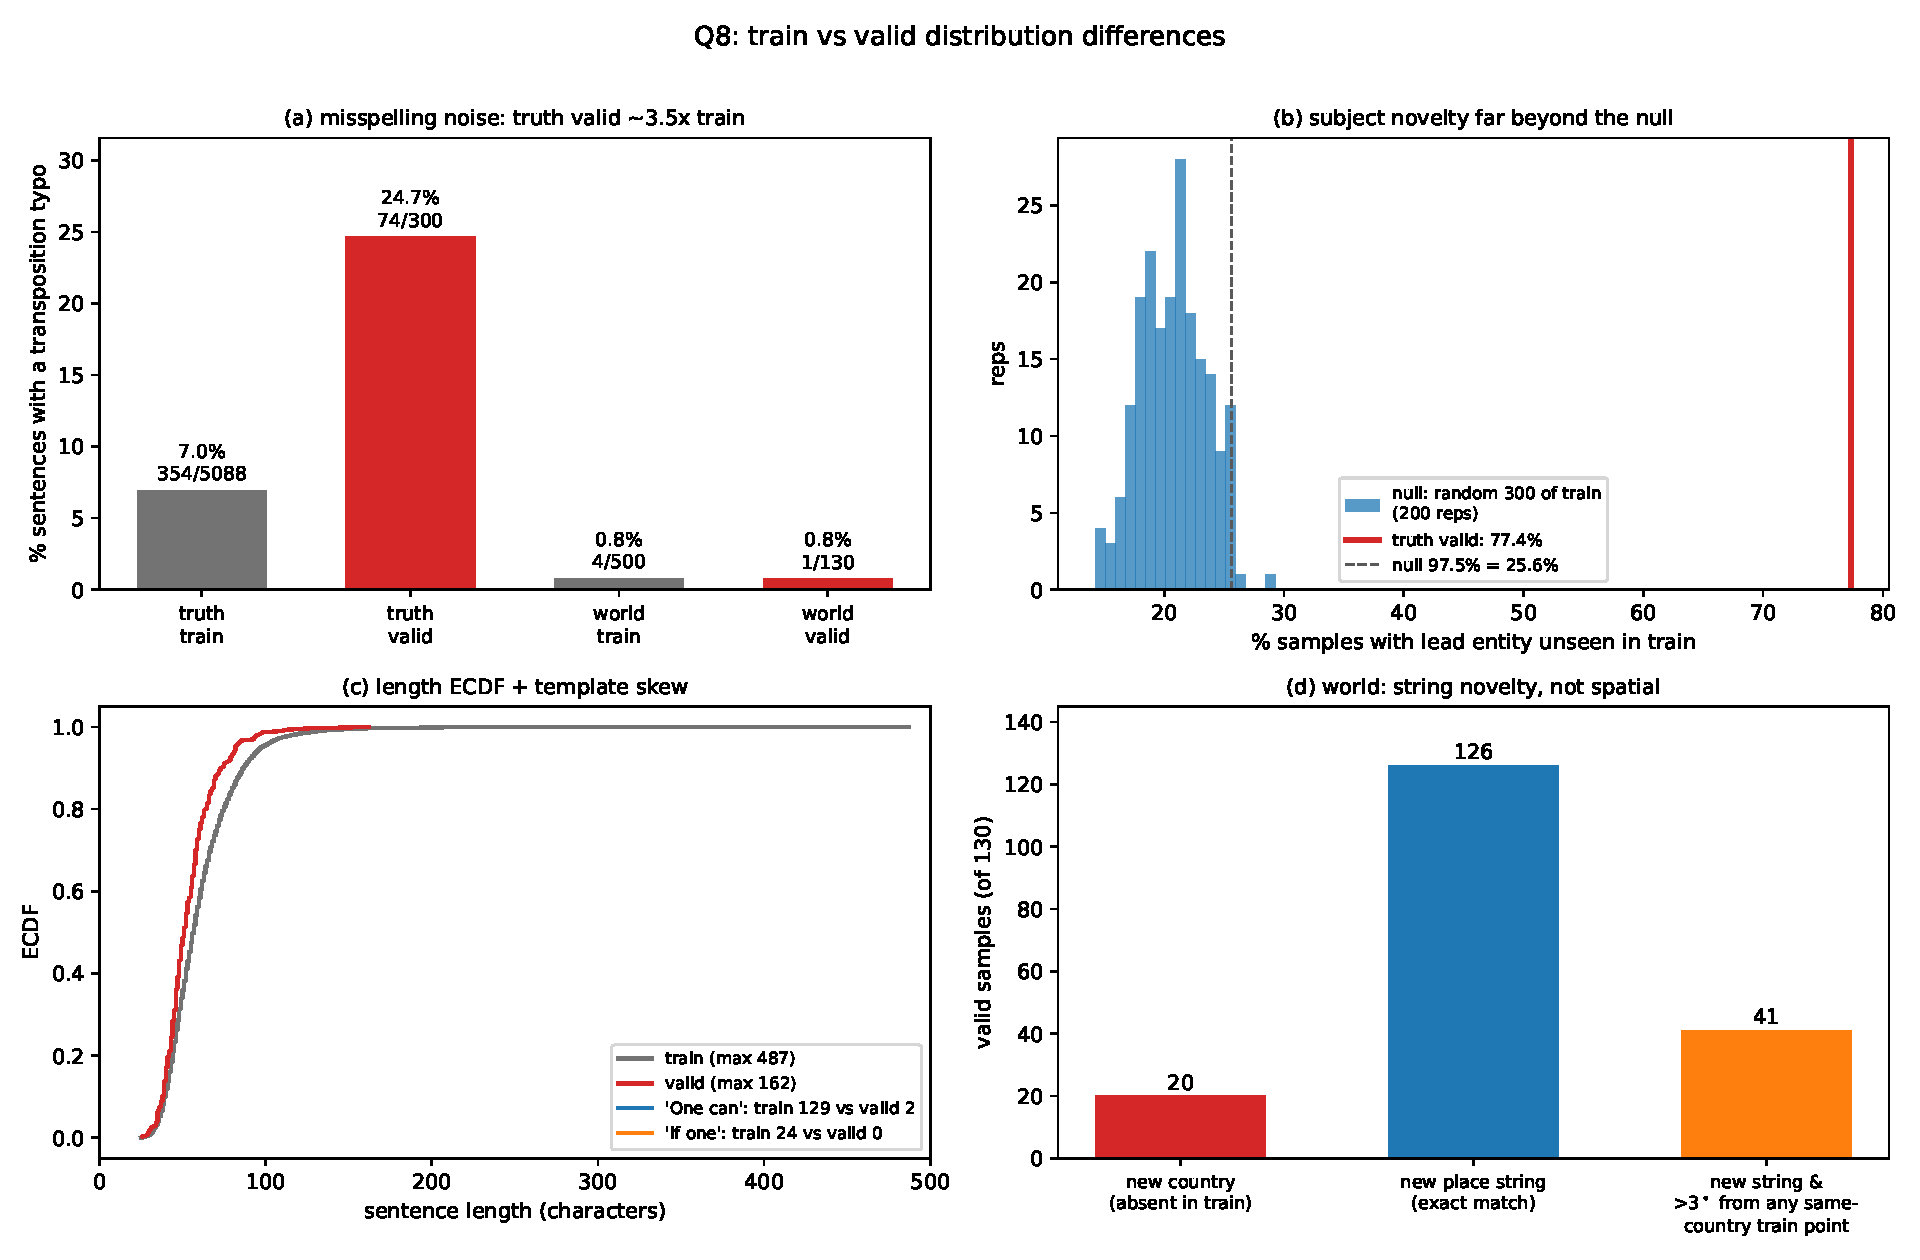
\includegraphics[width=\linewidth]{question/figures/q8_split_diff.pdf}
  \caption{分布差异总览：(a) 拼写噪声 valid $\approx$3.5$\times$ train；(b) 主体新颖度 77.4\% 远在零假设分布之外；(c) 长度 ECDF 与模板差异。}
\end{figure}

\begin{figure}[htbp]
  \centering
  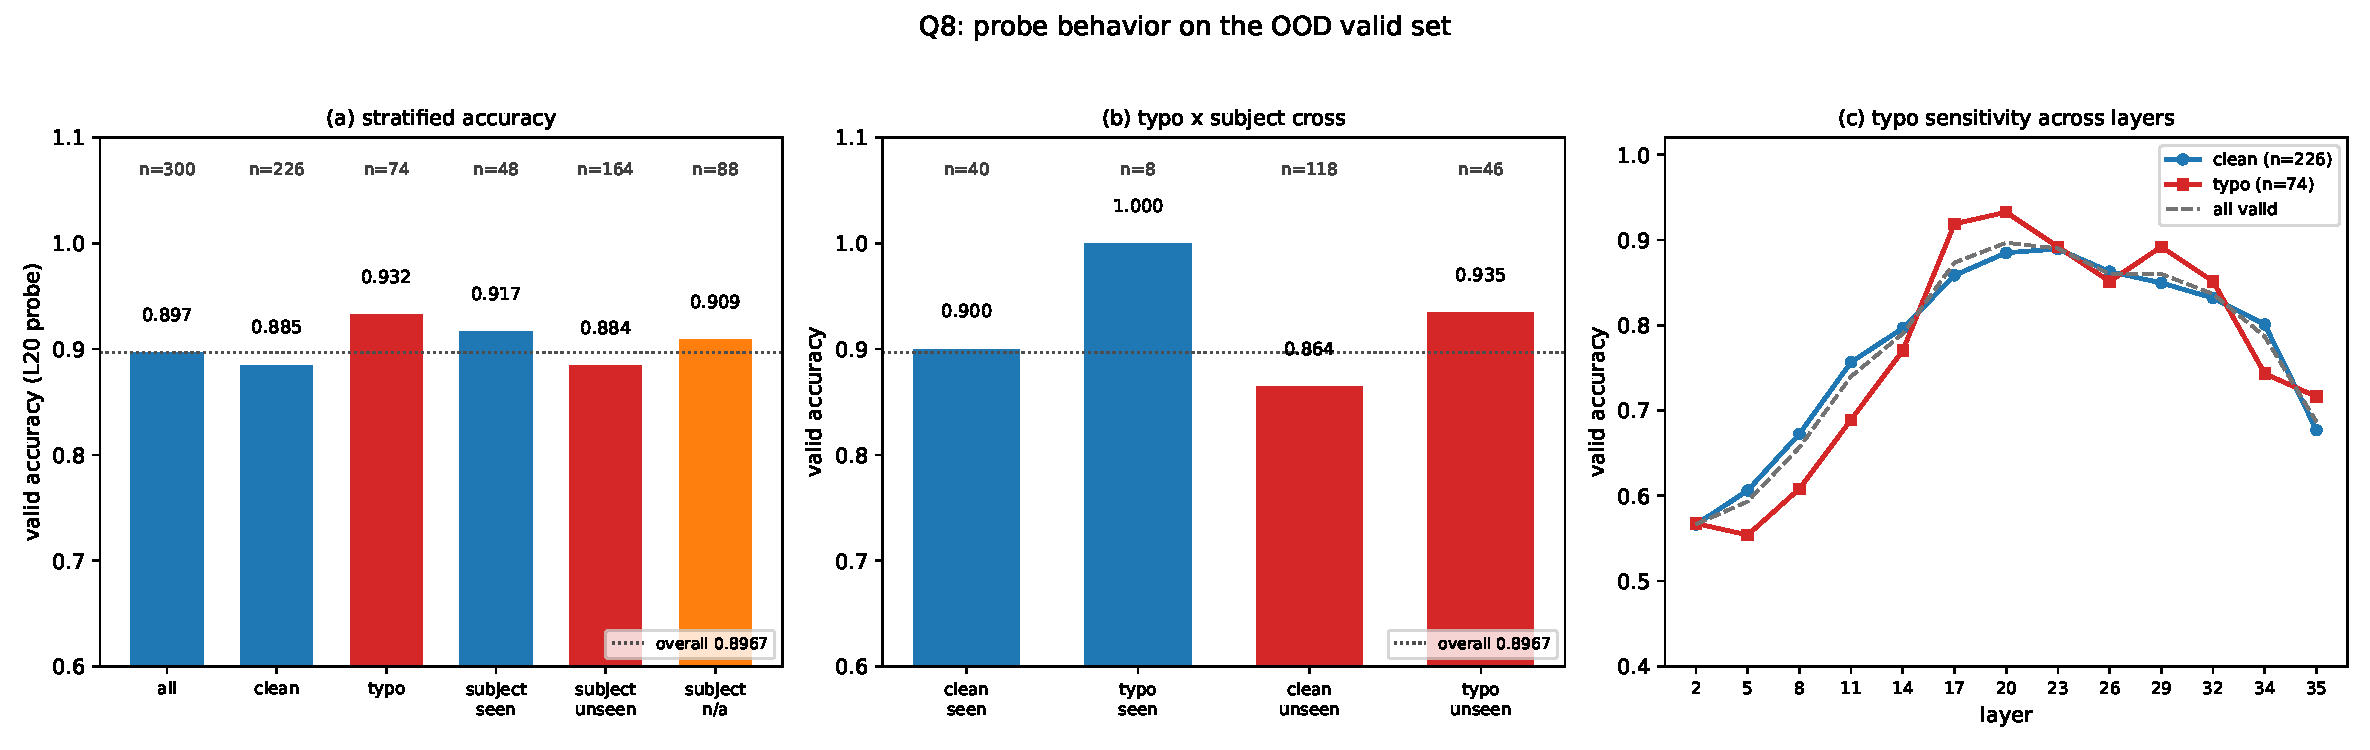
\includegraphics[width=\linewidth]{question/figures/q8_stratified_acc.pdf}
  \caption{L20 探针在 OOD valid 上的分层表现：(a) 主分层准确率；(b) typo $\times$ 主体交叉；(c) 13 层探针的 typo 敏感度。}
\end{figure}


% ======================================================================
\FloatBarrier
\subsection*{9. truth：选层与正则化的理由}

\textbf{题面：}你在最终模型提交中是怎么选择特征选取层次和正则化的？请说明理由。

\textbf{（1）实验设置。}和 world 一样扫 13 层，统一配置：lr$=5\times10^{-3}$、5000 轮、$\lambda_1=\lambda_2=10^{-3}$，truth 用原始特征，得到完整曲线。

\textbf{（2）结果分析。}truth 的曲线是清晰的\textbf{倒 U 形}：中间高、两边低。选 L20，因为它最高，而且峰位居中、两侧比较对称。解释：真假判断靠语义级信息，这些信息在 L17–L23 对线性探针最可读；浅层还是词法和局部特征，深层经过非线性重整后线索被稀释。这和 world 的最优层正好相反，说明不同深度装的是不同类型的信息。

\textbf{（3）正则化。}结果显示 $\lambda_1$ 有害：$0\to70.0\%$、$10^{-3}\to68.7\%$、$10^{-2}\to67.0\%$、$0.1\to\mathbf{50.0\%}$（直接掉到随机）。原因是表征稠密，$\ell_1$ 把大量分量压成 0，反而对准确率有害；$\lambda_2$ 则对准确率几乎无影响（四个取值都是 $68.7\%$）。所以最终取 $\lambda_1=\lambda_2=10^{-3}$，采用很弱的正则化。

\textbf{（4）最终提交。}\textbf{raw L20}，lr$=5\times10^{-3}$，5000 轮，$\lambda_1=\lambda_2=10^{-3}$，valid acc \textbf{0.8967}。

\begin{figure}[htbp]
  \centering
  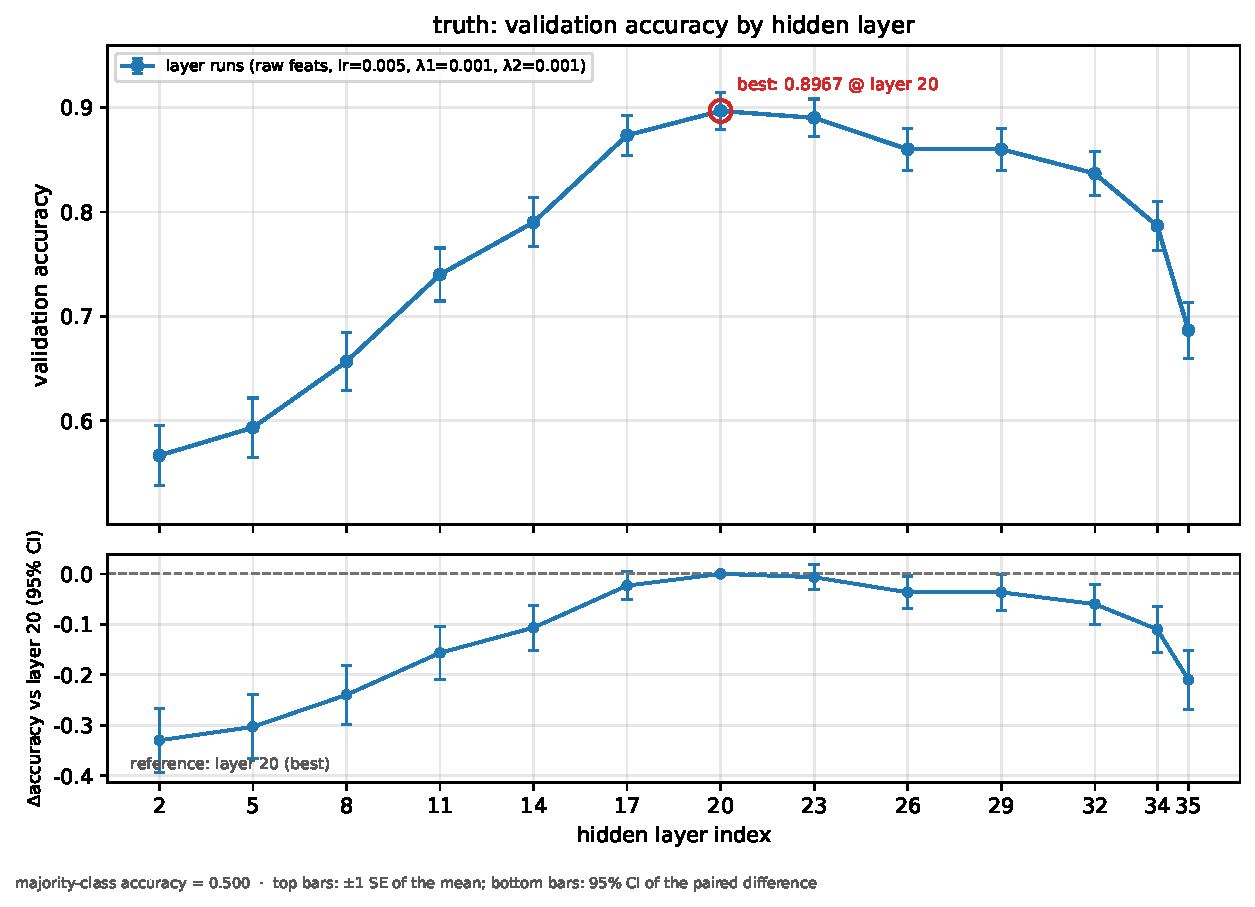
\includegraphics[width=\linewidth]{results/slurm_layers/truth/plots/truth_layers.pdf}
  \caption{truth 各层验证准确率（上：$\pm1$ SE，红圈 = L20；下：与 L20 的配对差 95\% CI）。倒 U 形、中层平台。随机水平 $=$ 多数类 $=0.50$。}
\end{figure}

\begin{table}[htbp]
  \centering
  \small
  \begin{tabular}{rrrl}
    \toprule
    层 & acc & $\pm$SE & $\Delta$ vs L20（95\% CI）/判定 \\
    \midrule
    2 & 0.5667 & 0.0287 & $-33.00$pp $\pm$ 6.36pp 显著 \\
    5 & 0.5933 & 0.0284 & $-30.33$pp $\pm$ 6.32pp 显著 \\
    8 & 0.6567 & 0.0275 & $-24.00$pp $\pm$ 5.88pp 显著 \\
    11 & 0.7400 & 0.0254 & $-15.67$pp $\pm$ 5.30pp 显著 \\
    14 & 0.7900 & 0.0236 & $-10.67$pp $\pm$ 4.47pp 显著 \\
    17 & 0.8733 & 0.0192 & $-2.33$pp $\pm$ 2.84pp 不显著 \\
    20 & \textbf{0.8967} & 0.0176 & 参考（最优） \\
    23 & 0.8900 & 0.0181 & $-0.67$pp $\pm$ 2.45pp 不显著 \\
    26 & 0.8600 & 0.0201 & $-3.67$pp $\pm$ 3.25pp 刚好显著 \\
    29 & 0.8600 & 0.0201 & $-3.67$pp $\pm$ 3.62pp 边缘 \\
    32 & 0.8367 & 0.0214 & $-6.00$pp $\pm$ 3.98pp 显著 \\
    34 & 0.7867 & 0.0237 & $-11.00$pp $\pm$ 4.50pp 显著 \\
    35 & 0.6867 & 0.0268 & $-21.00$pp $\pm$ 5.84pp 显著 \\
    \bottomrule
  \end{tabular}
  \caption{truth 13 层验证准确率全表（raw，lr$=5\times10^{-3}$，5000 轮，$n=300$）。}
\end{table}

\begin{figure}[htbp]
  \centering
  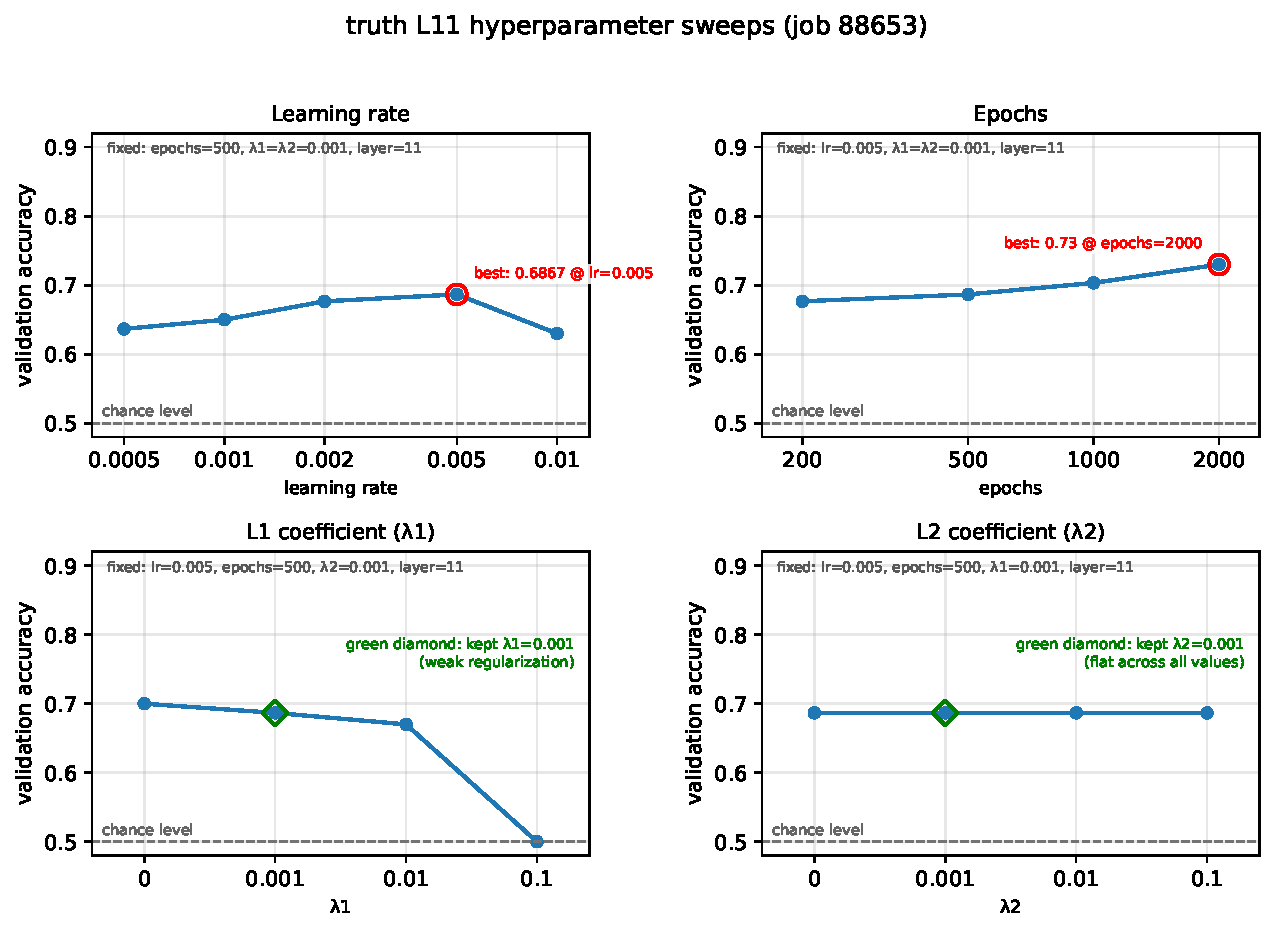
\includegraphics[width=\linewidth]{results/q9_grid/plots/truth_sweep.pdf}
  \caption{truth L11 超参数扫描（88653，原始特征，基线 lr$=5\times10^{-3}$、500 轮、$\lambda_1=\lambda_2=10^{-3}$，每格只变一个）：lr 呈倒 U，$5\times10^{-3}$ 最佳（68.7\%），$10^{-2}$ 回落到 63.0\%；epochs 在扫描范围内单调升（2000 轮 73.0\%，最终 13 层训练统一用 5000 轮）；$\lambda_1$ 从 $10^{-3}$ 增到 $0.1$ 时由 68.7\% 掉到随机水平 50.0\%（$0$ 时 70.0\% 略高，但无正则不稳定，故不取）；$\lambda_2$ 四个取值均为 68.7\%、完全不敏感。红圈为该格扫描最优，绿菱形为提交采用的 $\lambda_1=\lambda_2=10^{-3}$。}
\end{figure}


% ======================================================================
\FloatBarrier
\newpage
\appendix

% ======================================================================
\section{背景知识：线性探测、Qwen3-4B 与两个任务}\label{app:background}

线性探测（linear probing）[1] 是研究模型内部表征的一种回归分析手段：训练时冻结大语言模型，只在某一中间层的激活（隐表征）上训练一个简单模型——本实验中即手写实现的线性回归与逻辑回归；若该模型能在独立验证集上优于合理基线，说明相应信息以（近似）线性可分的形式编码于该层表征、可被“解码”。线性可解码是一个良好的性质：信息可用简单模型读出，也是激活引导（activation steering）等后续干预研究的前提；但需注意“可解码 $\neq$ 模型在生成时一定使用了该信息”。本实验考察 Qwen3-4B-Base 内部的两类表征：地理空间坐标（论文 [3] 实验的简化，用线性回归预测经纬度）与句子真假（论文 [4] 实验的简化，用逻辑回归预测真假标签）。

特征口径：Qwen3-4B-Base 共 36 个 decoder block（编号 0–35），隐藏维度 $D=2560$；特征取指定词元在 block 输出处（最终 RMSNorm 之前）的隐状态，不使用聊天模板。词元选择随任务而定：world 取“国名最后一个词元”，truth 取“句子最后一个词元”。课程预提取了第 11、23、35 层；我们另按实验文档的算力平台教程提取了其余 10 层，凑成 13 层（从 2 到 35、步长约 3）以支撑层间对比（提取与训练的工程细节见附录~\ref{app:exp}）。特征文件以 float16 存储为 $(N,2560)$ 数组，训练与评测时转为 float64。

两个任务的规模与角色不同。world 为回归任务（热身）：train 500 / valid 130，目标为（纬度, 经度）双输出（单位度，北纬、东经为正），按 MSE 评测；$N=500\ll D=2560$ 为欠定问题，必须借助正则化与特征层选择获得泛化能力，课程对其效果赋权低于 truth。truth 为二分类任务（主考察）：train 5088 / valid 300，标签 1 为真、0 为假，两个集合内真假各半；样本数大于特征维度。两者的最终效果均在一个未公布的测试集上评测，且测试集分布更接近验证集而非训练集——因此不应以过拟合训练集的方式提分。

提交物为两份 \texttt{.npz} 权重（\texttt{float64}）：world 为 \texttt{weights} $(2,2560)$（两行依次对应纬度、经度）与 \texttt{bias} $(2,)$；truth 为 \texttt{weights} $(2560,)$ 与零维 \texttt{bias}；另附所选特征层的层号（$[0,35]$ 整数）。两个数据集均为课程自建、与论文原实验所用不同，构造细节未公布；关于它们的构造线索与训练/验证分布差异，见第 8 题。


% ======================================================================
\section{有意思的实验：超参数扫描、稳定界与工程实践}\label{app:exp}

在正式的分层训练之前，我们做了两轮系统性的超参数扫描（全部为全批量 GD、确定性代码，本地与集群数值一致）。首轮（job 88653）以单变量对照的形式跑了 9 组 35 次训练：两任务在 L11 上分别扫 lr、epochs、$\lambda_1$、$\lambda_2$，并以 L11/23/35 扫描层。扫描给出的主要结论与正文 Q5/Q9 一致，此不重复；这里值得记录的是扫描本身暴露出的形态：truth 的 lr 呈倒 U（0.005 最佳）、$\lambda_1$ 有害、层间差异巨大（L23 84.3\% 对 L11/L35 的 63\% 上下）；world 则是 lr 越大越好但上限被锁死在 $5\times10^{-4}$（150.94），layer 23/35 在 lr$=2\times10^{-4}$ 下直接发散为 inf——同一份扫描在两个任务上呈现完全不同的数值面貌（logistic 有界梯度对 MSE 无界残差），由此引出了一整条“数值修复”支线。

world 的发散最初表现为一串极具误导性的日志与状态。日志写“Training converged at epoch 263, loss=inf”——收敛判据 \texttt{np.isclose(inf, inf)} 为真，把损失溢出误报成了收敛；实测权重并未变成 nan，而是有限的天文数字（max$|w|$ 达 $1.8\times10^{151}$、$7.9\times10^{152}$），旧代码“权重是否有限”的检查因此误报通过；更隐蔽的是发散时预测出的 MSE 是有限大数（$3.9\times10^{305}$）而非 inf——“只查权重”或“只查指标”都会漏检，必须引入独立的发散标志位。

修复分三处：\texttt{model.py} 新增 diverged 状态（梯度/权重/loss 非有限、或 loss 超过初始值 $10^6$ 倍即中止训练并置位，与正常收敛严格区分）；\texttt{run\_grid.py} 支持逐组 standardize（z-score 统计量只取 train split、验证集复用同一 $\mu/\sigma$），并支持把标准化空间的权重精确折回原始特征空间（$w'=w/\sigma$、$b'=b-\mu\cdot w'$，在原始特征上复算一致、误差 $\sim10^{-14}$）。根因也随之明确：发散不是“深层没有信息”，而是 lr 越过了\textbf{按层稳定界}——未标准化时该界随深度暴跌 1800 倍（数学见附录~\ref{app:math}）。

第二轮（job 89085，16 次训练）在 z-score 特征上重扫。标准化把各层稳定界拉平后，lr$=3\times10^{-3}$ 对三层均安全、$5\times10^{-3}$ 的越界被 \texttt{finite=False} 正确标记为发散；$\lambda_2$ 呈现出真实的 U 形（$0.1\to209.13$——训练已收敛但验证严重过拟合；$1.0\to167.06$ 最优；$3.0\to184.57$）；epochs $\ge500$ 即到平台。layer 扫描（lr$=3\times10^{-3}$）：L11 167.06 / L23 241.12 / L35 204.98。$\lambda_1$ 另外补扫 4 点（同一 std L11 配置，$0,10^{-3},10^{-2},0.1$）：MSE 分别为 $167.07,167.06,166.93,165.82$，$0.1$ 相对 $10^{-3}$ 的配对差为 $-1.24$（95\% CI $[-5.80,3.33]$），不显著。至此三条独立路径——raw 冠军（L11 150.4）、raw 长训练（L23 在 lr$=5\times10^{-5}$、20000 轮下 233.1）、标准化收敛（上列数字）——交叉印证了“L11 是 world 最优层、L23/35 在真正收敛后确实更差”，排除了“深层只是训不动”的假象。

工程方面，truth 的“13 层 $\times$ 5000 轮”在 4h 平台上限内跑不完（首跑 89700 超时），我们把它拆成 4 个分块作业（90243–90246）并实现断点续跑：\texttt{-{}-skip-existing} 复用已完成层、\texttt{python -u} 实时日志、BLAS 线程钉定避免共享节点抢占。四个作业全部成功、零发散；L5 撞上慢节点跑了 3390.5s（约 15 倍于正常耗时）仍被分块设计吸收、零进度损失。统计方法上，层间比较统一使用同批验证样本的\textbf{配对 bootstrap 95\% CI}：world 的 MSE 重尾，单层 SE 达 40+，配对后 CI 显著收窄（25–77）；truth 单样本值 0.33pp。

\begin{figure}[htbp]
  \centering
  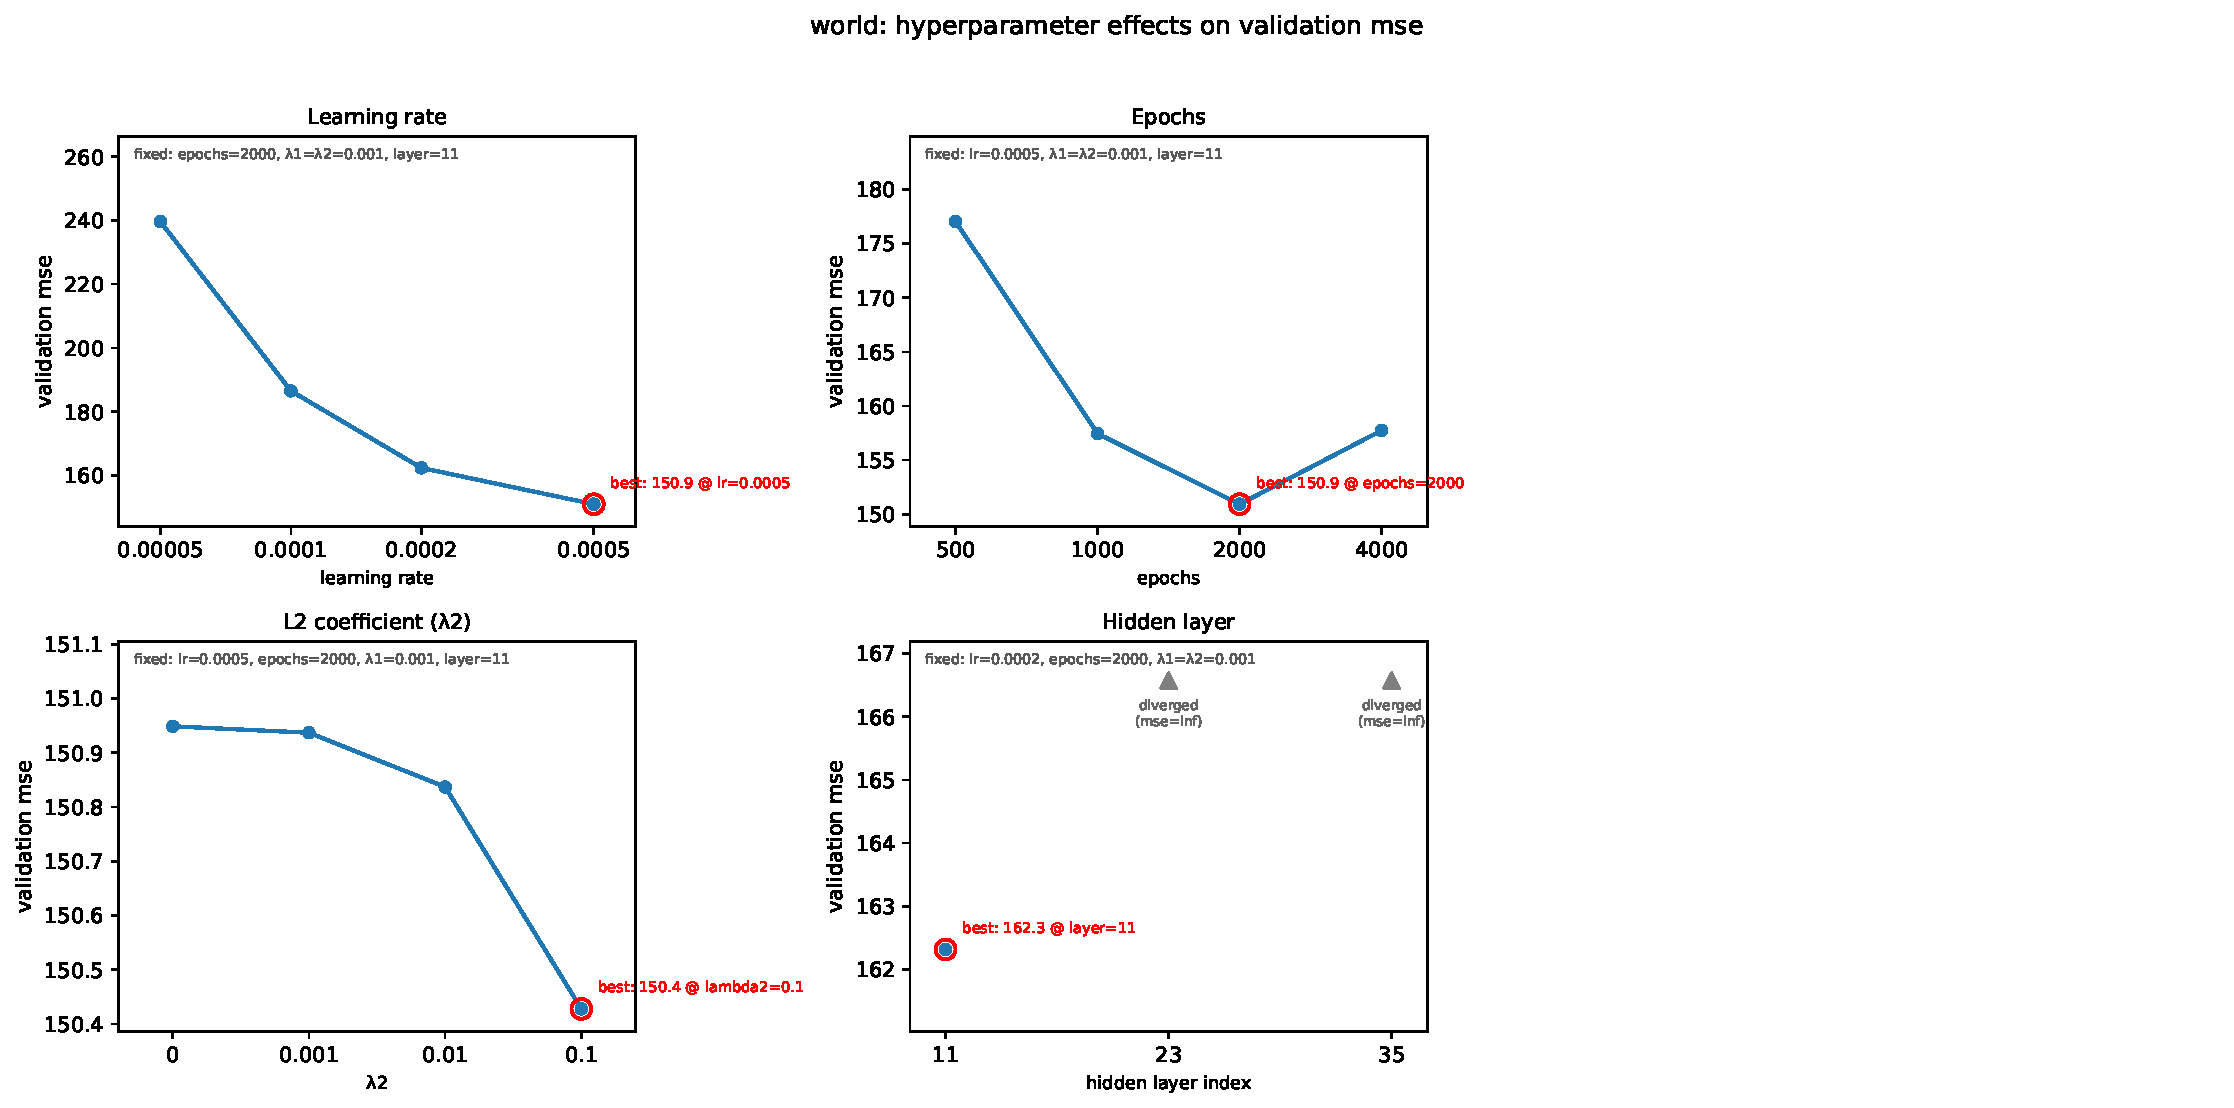
\includegraphics[width=\linewidth]{results/slurm_grid/20261009_115559_88653/plots/world_grid.pdf}
  \caption{首轮 world 超参数扫描（88653，未标准化特征）：lr 越大越好但上限被困在 $5\times10^{-4}$（更大即发散）；layer 23/35 的“inf”由数值问题造成，而非“深层无信息”。}
\end{figure}

\begin{figure}[htbp]
  \centering
  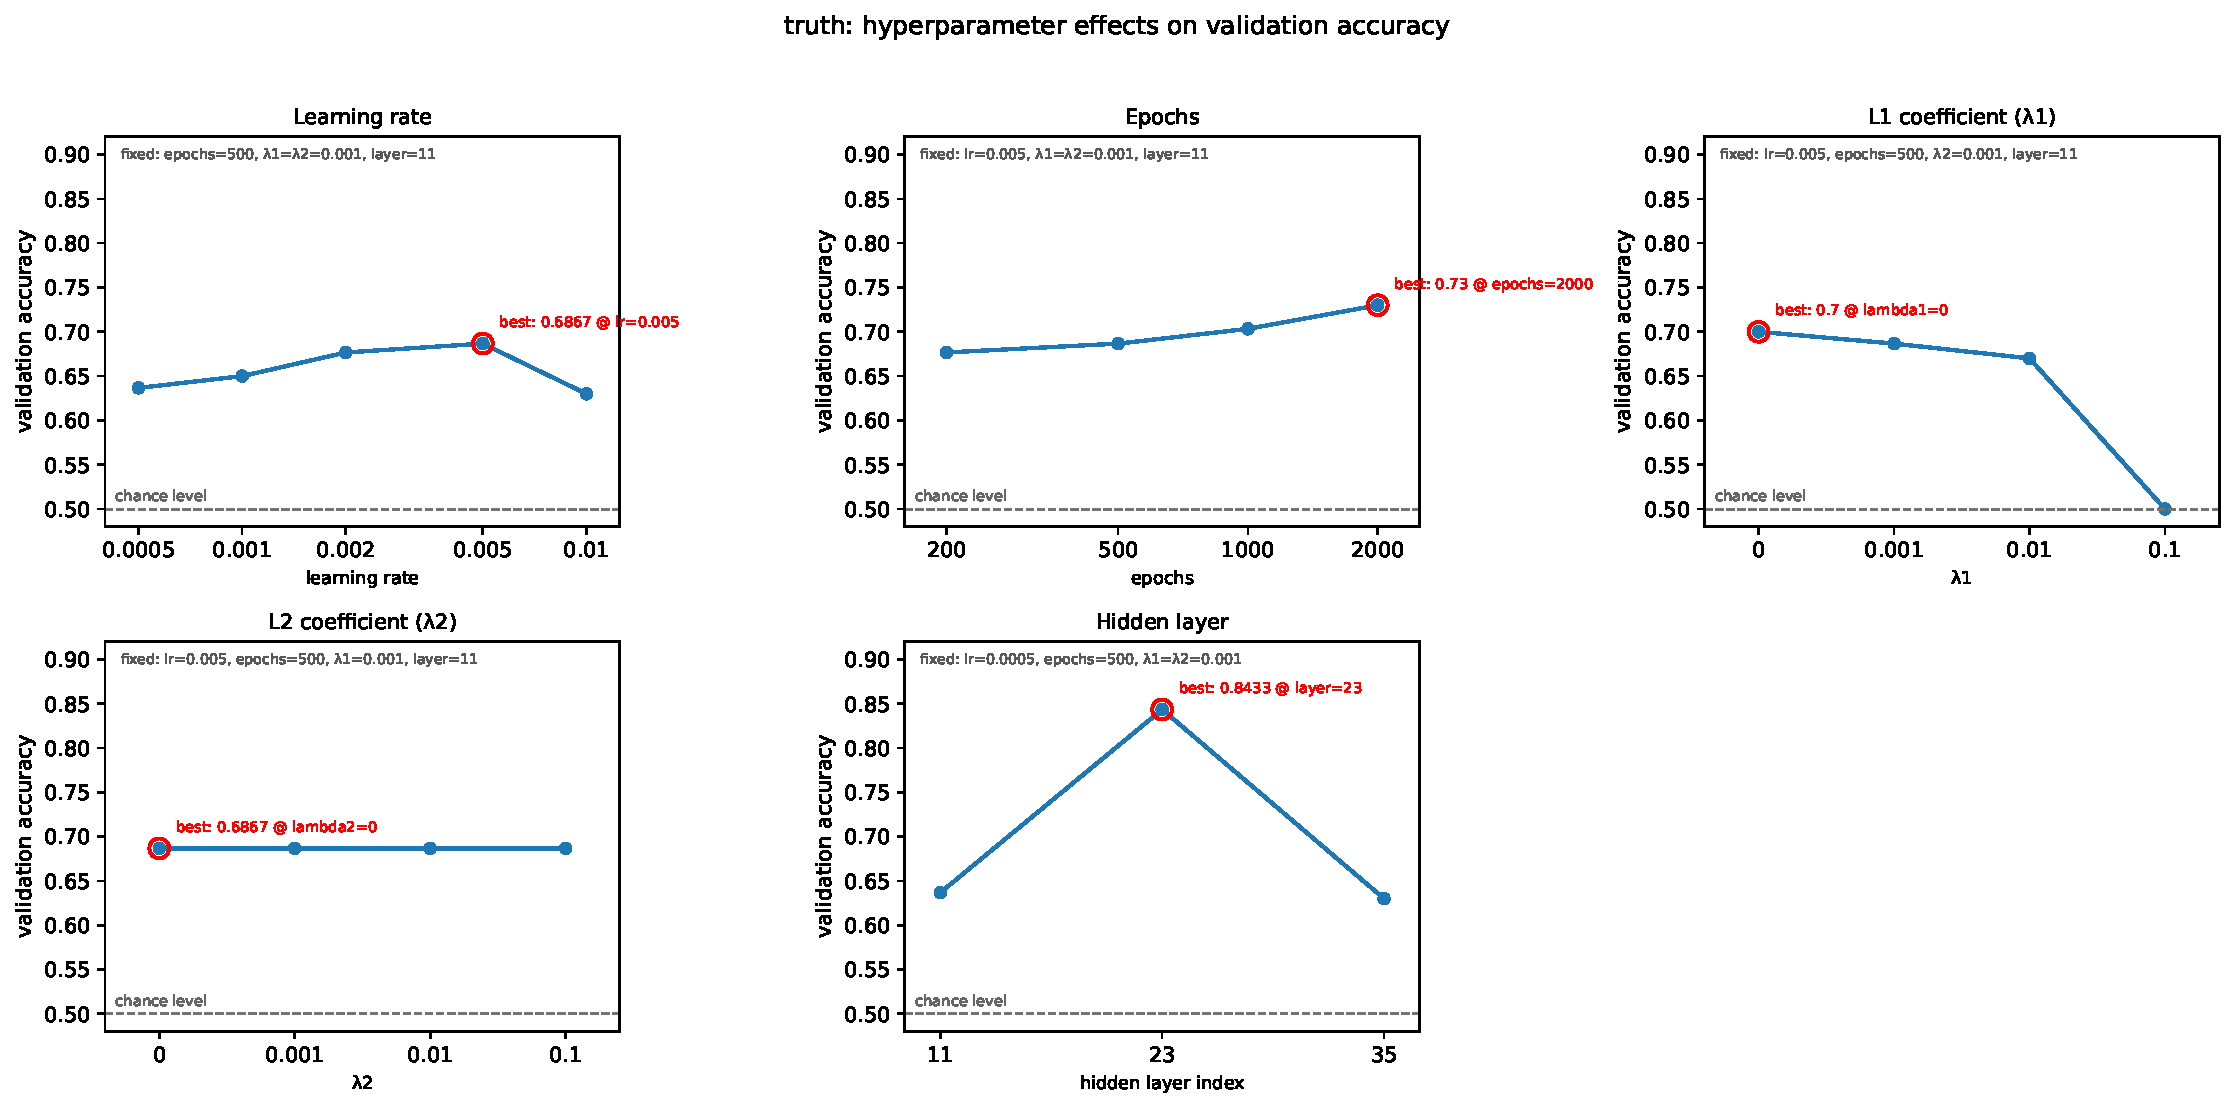
\includegraphics[width=\linewidth]{results/slurm_grid/20261009_115559_88653/plots/truth_grid.pdf}
  \caption{首轮 truth 超参数扫描（88653）：lr、epochs、layer 的效应；$\lambda_1$ 增大有害、$\lambda_2$ 无差异。}
\end{figure}


% ======================================================================
\section{有趣的表征：跨任务对照与现象观察}\label{app:repr}

本附录收集正文放不下的跨任务表征观察与现象汇总。第一，两任务的\textbf{最优层带完全不同}：world 在浅层 L2–L11（157.6–167.0 的平台），truth 在中层 L17–L23（0.8733–0.8967 的平台），且两者都在 L32–L35 变差——位置/坐标信息与真假语义的“可线性解码深度”不同，说明不同类型的信息写在表征的不同深度上。一处与论文的差异如实报告：论文 [3] 在 LLaMA-70B 上报告 world 表征约在 60\% 深度处最佳，而我们在 Qwen3-4B 上的 world 最优却在很浅的层——模型、数据集与特征口径均不同，我们不做进一步归因。

第二，raw 与 z-score 的相互作用是一个非平凡的观察：raw 特征的增益并非“浅层普遍更好”，而是 L11 特有的组合——raw L11 全场最低（150.43），但 raw L2 探针反而显著更差（198.78）；z-score 的意义也不是“提点”，而是\textbf{解锁深层}——把按层稳定界拉平（1800 倍差距缩到 1.5 倍）让深层可训，同时 L2 的浅层优势本身也依赖标准化解锁（raw 198.8 $\to$ std 157.6）。

第三，一个只报告、暂不归因的现象：world 的曲线在深层\textbf{回升}——从 L20/L23 的低谷（$\approx241$）回到 L32 的 180.3、与浅层统计不可区分（L11 vs L32：t$=-0.46$；而 L23 vs L32 的回升在配对意义上显著）；truth 则没有这个现象，L26 起单调下降（L32 的 0.8367 $\to$ L35 的 0.6867）。两任务在尾部层的表现分化，其机制（残差流叠加读出、语义抽象稀释等解释）都在本实验证据之外，我们只报告观察。

第四，把 Q6–Q8 的表征现象汇总：坐标信息以超越国家身份的形式存在——unseen 20 条上 improvement $+1023.93\ [513.94,\ 1654.14]$（这些国家按表查询在原理上不可能）；同国内纬度弱可解码（$r=0.201$）、经度近乎不可解码（$r=0.046$），与 Q6 地图上“经度误差 $\gg$ 纬度”（MAE 10.85$^\circ$ vs 4.25$^\circ$）相互印证，共同指向“气候带式”的粗粒度空间信息与有限的地名知识。噪声维度上，中深层表征对字符级扰动不敏感（typo 子集 acc 不低于 clean，浅层 L5–L11 才有 5–7pp 的差距）——与“表征是分布式语义编码”的直觉一致。

第五，一条 token 口径备注：world 探针读的是“国名最后一个词元”处的激活——写入位置即国家实体本身的状态；结果表明该状态同时编码了超越国名的坐标信息（否则 unseen 国家上不可能大幅胜过全局基线）。这也可能与 Q7 观察到的“国家中心收缩”有关：从国名词元状态读出的位置天然带有国家先验，探针只能部分解出个体地点的偏移。


% ======================================================================
\section{数学原理：稳定界、闭式解与 KKT}\label{app:math}

world 用均方误差 $L=\|Xw+b\mathbf 1-y\|^2/N$（与 \texttt{model.py} 一致），它是关于参数的凸二次函数，Hessian $H=2X^{\top}X/N$。全批量梯度下降的误差传播为 $e_{t+1}=(I-\mathrm{lr}\,H)e_t$（$e$ 为参数误差），收敛当且仅当谱半径小于 1，即 $\mathrm{lr}<\dfrac{2}{\lambda_{\max}(H)}=\dfrac{N}{\|X\|_2^2}$——只依赖特征矩阵、与 $y$ 无关，每层各有一个值（$N$ 为该任务训练样本数）。越界后，误差沿最大特征方向每轮乘以 $|1-\mathrm{lr}\,\lambda_{\max}|>1$ 指数放大——这正是 world 未标准化时 loss 奔向 inf 的机制。

truth 用交叉熵，其 Hessian 为 $X^{\top}\mathrm{diag}(p(1-p))X/N\preceq X^{\top}X/(4N)$，最坏情形（$p=1/2$）的充分稳定界放宽到约 $8N/\|X\|_2^2$（二次界的 8 倍）；更重要的是 logistic 的梯度有界（$p-y\in[-1,1]$），没有 MSE“残差随 $w$ 线性增长”的正反馈，越界一般表现为震荡/饱和、准确率下降，而不是爆炸——这是 truth 可以不标准化、直接用 raw 特征配 lr$=5\times10^{-3}$ 的原因。

下表给出 13 层 $\times$ 两任务 $\times$ raw/z-score 的全部稳定界，两个读法。其一，\textbf{raw 界随深度暴跌}——world 从 L2 的 $4.95\times10^{-3}$ 降到 L35 的 $2.77\times10^{-6}$，跨约 1800 倍；激活幅度逐层增大（残差流行范数从 51 到 623，约 12 倍，平方进入 $\|X\|_2^2$ 就是两个数量级），固定 lr 必然在深层越界。其二，\textbf{z-score 把界“拉平”}到 $3.1$–$4.8\times10^{-3}$（仅 1.5 倍差距）——z-score 只归一化每列尺度，剩下的差异来自特征间的相关结构；正因为拉平了，同一个 lr 才能对所有层公平。truth 的 raw 界同样随深度收缩，但如上所述 logistic 对越界是“软”的，其配置不依赖这把尺子。

\begin{table}[htbp]
  \centering
  \small
  \begin{tabular}{rrrrr}
    \toprule
    层 & world raw & world z-score & truth raw & truth z-score \\
    \midrule
    2 & $4.95\times10^{-3}$ & $4.07\times10^{-3}$ & $6.51\times10^{-3}$ & $2.67\times10^{-3}$ \\
    5 & $1.14\times10^{-3}$ & $\mathbf{3.08\times10^{-3}}$ & $1.14\times10^{-3}$ & $4.85\times10^{-3}$ \\
    8 & $6.90\times10^{-4}$ & $3.15\times10^{-3}$ & $1.09\times10^{-3}$ & $9.20\times10^{-3}$ \\
    11 & $5.45\times10^{-4}$ & $3.59\times10^{-3}$ & $7.37\times10^{-4}$ & $9.74\times10^{-3}$ \\
    14 & $4.47\times10^{-4}$ & $3.40\times10^{-3}$ & $6.10\times10^{-4}$ & $1.05\times10^{-2}$ \\
    17 & $3.19\times10^{-4}$ & $3.48\times10^{-3}$ & $5.01\times10^{-4}$ & $1.03\times10^{-2}$ \\
    20 & $1.93\times10^{-4}$ & $3.42\times10^{-3}$ & $3.04\times10^{-4}$ & $7.00\times10^{-3}$ \\
    23 & $8.37\times10^{-5}$ & $3.16\times10^{-3}$ & $1.33\times10^{-4}$ & $5.38\times10^{-3}$ \\
    26 & $3.94\times10^{-5}$ & $3.16\times10^{-3}$ & $4.08\times10^{-5}$ & $4.72\times10^{-3}$ \\
    29 & $1.89\times10^{-5}$ & $3.46\times10^{-3}$ & $1.63\times10^{-5}$ & $5.42\times10^{-3}$ \\
    32 & $7.48\times10^{-6}$ & $3.92\times10^{-3}$ & $6.17\times10^{-6}$ & $6.70\times10^{-3}$ \\
    34 & $3.02\times10^{-6}$ & $4.40\times10^{-3}$ & $2.93\times10^{-6}$ & $7.25\times10^{-3}$ \\
    35 & $2.77\times10^{-6}$ & $\mathbf{4.77\times10^{-3}}$ & $1.68\times10^{-6}$ & $5.84\times10^{-3}$ \\
    \bottomrule
  \end{tabular}
  \caption{13 层稳定界 $N/\|X\|_2^2$ 全表（SVD 精确值；raw 界随深度跨 1800$\times$，z-score 后压至 1.5$\times$）。}
\end{table}

理论与实测逐条吻合：raw L11 界 $5.4\times10^{-4}$——lr$=5\times10^{-4}$ 稳定（贴线，MSE 150.9），$10^{-3}$ 直接溢出；raw L23 界 $8.4\times10^{-5}$——实测 $2\times10^{-4}$（超 2.4 倍）收敛前爆炸；raw L35 界 $2.8\times10^{-6}$——实测超 72 倍、71 轮即炸；std L11 界 $3.6\times10^{-3}$——lr$=3\times10^{-3}$（0.83 倍）得 167.06、$5\times10^{-3}$（1.39 倍）发散；std L35 界 $4.8\times10^{-3}$——lr$=4\times10^{-3}$（0.84 倍）冒烟 300 轮稳定、$8\times10^{-3}$（1.68 倍）第 9 轮爆炸。反向一例：truth raw L35 用 lr$=5\times10^{-4}$ 已超二次界约 300 倍，训练仍然有限（acc 63.0\%）——logistic 的非爆炸性由此得到实证。

Q1/Q2 的实现用到两条精确算法。其一，Ridge 的 SVD 闭式解：$X=U\Sigma V^{\top}$ 时 $\hat w= V\,\mathrm{diag}\!\big(\sigma_i/(\sigma_i^2+\lambda)\big)\,U^{\top}y$，$\lambda=0$ 退化为伪逆的最小范数最小二乘解；系数路径即由它精确计算（与 sklearn 对拍 $10^{-9}$）。其二，Lasso 的 KKT/软阈值：驻点条件 $\partial L/\partial w_j=\frac{2}{N}[X^{\top}(Xw-y)]_j+\lambda_1\, \mathrm{sgn}(w_j)+2\lambda_2 w_j=0$ 由坐标下降 $+$ warm start 求解；精确零来自优化几何本身、零集沿 $\lambda$ 嵌套——这正是 Q2 中“阈值化 ridge 无法复现 lasso 零集”对照的数学背景。逻辑回归的梯度（\texttt{model.py} 实现）为 $\nabla_w L=\frac{1}{N}X^{\top}(\hat y-y)+\lambda_1\,\mathrm{sgn}(w)+2\lambda_2 w$；数值上用 $\log(1+e^{-z})=\mathrm{logaddexp}(0,-z)$ 稳定计算。sklearn 换算表（Q3 对拍用）：Ridge $\alpha=N\lambda_2$；Lasso $\alpha=\lambda_1/2$；ElasticNet $\alpha\rho=\lambda_1/2$、$\alpha(1-\rho)=\lambda_2$；Logistic $C=1/(2N\lambda_2)$——注意 sklearn 的正则量纲是“平方误差总和”口径，直接对比会差一个 $N$ 倍。最后是基线口径：train 均值基线的元素平均口径 MSE $=3311.27$（与模型指标同口径），坐标求和口径 $=6622.54$；两者混用会把 $R^2$ 抬高约 2.3pp。统一口径后，world 最佳 $R^2=0.9546$（RMSE $\approx$ 12.3$^\circ$）。


% ======================================================================
\section{复现清单与文件结构}\label{app:repro}

本报告的仓库结构与产物分布如下。根目录的 \texttt{model.py} 是提交的手写模型（线性/逻辑回归，全批量梯度下降）；\texttt{datasets/} 存放两任务各 13 层的特征数组与标签 csv；\texttt{experiments/} 是训练与分析的执行器与配置（\texttt{train\_layers.py}、\texttt{run\_grid.py}、\texttt{plot\_layers.py}、\texttt{stability\_bound.py} 及配置 json）；\texttt{scripts/} 是集群 sbatch 与分块提交脚本；\texttt{question/code} 是思考题 Q1–Q8 的复现脚本；\texttt{results/} 汇总全部扫描/分层训练/提取的结果与图；\texttt{report/} 为本报告源文件。

环境方面，本地与集群统一使用 ai26 环境（numpy / sklearn / matplotlib / cartopy / pyspellchecker）；集群跑在 Students 分区，且必须钉 A100（\texttt{-{}-gres=gpu:A100:1}）——RTX5090 节点与当前 torch 驱动不兼容，需避开。关键复现命令：训练 13 层 \texttt{python experiments/\allowbreak train\_\allowbreak layers.py --skip-\allowbreak existing}；稳定界全表 \texttt{python experiments/\allowbreak stability\_\allowbreak bound.py}；Q1 系数路径 \texttt{python question/\allowbreak code/\allowbreak q1\_\allowbreak coefficient\_\allowbreak paths.py}；Q6 地图 \texttt{python question/\allowbreak code/\allowbreak q6\_\allowbreak valid\_\allowbreak map.py}；其余思考题脚本同构（入口在 \texttt{question/code} 下）。

提交产物（首选/备选）：world——raw L11 探针（\texttt{results/\allowbreak slurm\_layers/\allowbreak world/weights/\allowbreak world\_layer11\_extra0/\allowbreak weights.npz}，MSE 150.43），备选 z-score L2（157.57）；truth——raw L20（\texttt{results/\allowbreak slurm\_layers/\allowbreak truth\_b/weights/\allowbreak truth\_layer20/\allowbreak weights.npz}，acc 0.8967），备选 L23（0.8900）。所有权重均已折回原始特征空间，推理时不需再做标准化。

追溯与归档：KC 房价数据（Q1/Q2）与 OpenML 全表的逐格对拍记录在 \texttt{question/\allowbreak execution\_\allowbreak log.md} §1.2；truth 数据集的来源指纹见第 8 题；每轮集群运行的全部日志按时间戳归档在 \texttt{results/\allowbreak slurm\_*} 对应目录下。

% ======================================================================
\section{实验反馈与建议}\label{app:feedback}

全程做下来，我们对课程设计有几点想反馈。数据集构造不公布反而促成了本报告中最有意思的一段工作——Q8 的“反推/对拍”（用统计指纹识别出 valid 是构造性 OOD 挑战集）。我们建议在指南中明确鼓励这类来源调查：它把“调参竞赛”变成了真正的研究过程。报告要求“思考题回答为主、背景进附录、不设长度限制”的设定也很好，让扫描、稳定性分析等附加内容可以放进附录而不挤压正文；提示中“推荐 AI 工具辅助可视化”明确而友好，建议再补充一句“AI 辅助内容需能讲清原理”（验收提示已有类似要求）。

算力平台方面有两个具体的坑与建议。其一，Students 分区混部 RTX5090 与 A100，当前 torch 与 RTX5090 驱动不兼容（CUDA error 804），曾让整批特征提取全部 FAIL；建议在附录 B 的教程里明确写“钉 A100”。其二，4h 作业时限对“13 层 $\times$ 5000 轮”级别的实验需要分块 + 断点续跑设计——这本身是一次很好的工程训练（我们靠它吸收了慢节点 15 倍的抖动），但建议指南给出各量级实验的时间预算参考，避免每个小组都从超时失败学起。

\end{document}
